\documentclass[../../compsys.tex]{subfiles}
\begin{document}
\chapter{L4 - Memory}
\textit{This chapter covers the fundamentals of main memory, process memory images, memory virtualization, and the CPU's role in managing memory.}
\vspace{15px}
\section{Main Memory}
Main memory is conceptualized as a linear array of bytes, where each byte has a unique memory address (e.g., \texttt{0x0}, \texttt{0x1}, \texttt{0x2}, etc.). Each byte can store any value that fits within its 8-bit capacity, and importantly, the value stored in a given byte is independent of its memory address. For instance, the byte at address \texttt{0x0} may contain the value 8, 0, or any other valid 8-bit number.

\subsection{Memory Operations by the CPU}
The CPU interacts with main memory by executing specific instructions to read from and write to it. These operations are fundamental to both data processing and code execution:

\begin{itemize}
  \item[-] \textbf{Read Operation:} The CPU issues an instruction to read a block of bytes (for example, 8 bytes starting at address \texttt{0x0}) and loads the result into a register (such as \texttt{rax}).
  \item[-] \textbf{Write Operation:} The CPU executes an instruction that writes data from a register (e.g., \texttt{rax}) into a block of memory (for example, starting at address \texttt{0xb}).
\end{itemize}

Although main memory stores only numbers, the CPU interprets these numbers differently depending on whether they represent data (such as variables) or executable code (such as the instruction \texttt{mov rax, [0x0]}).

\begin{center}
  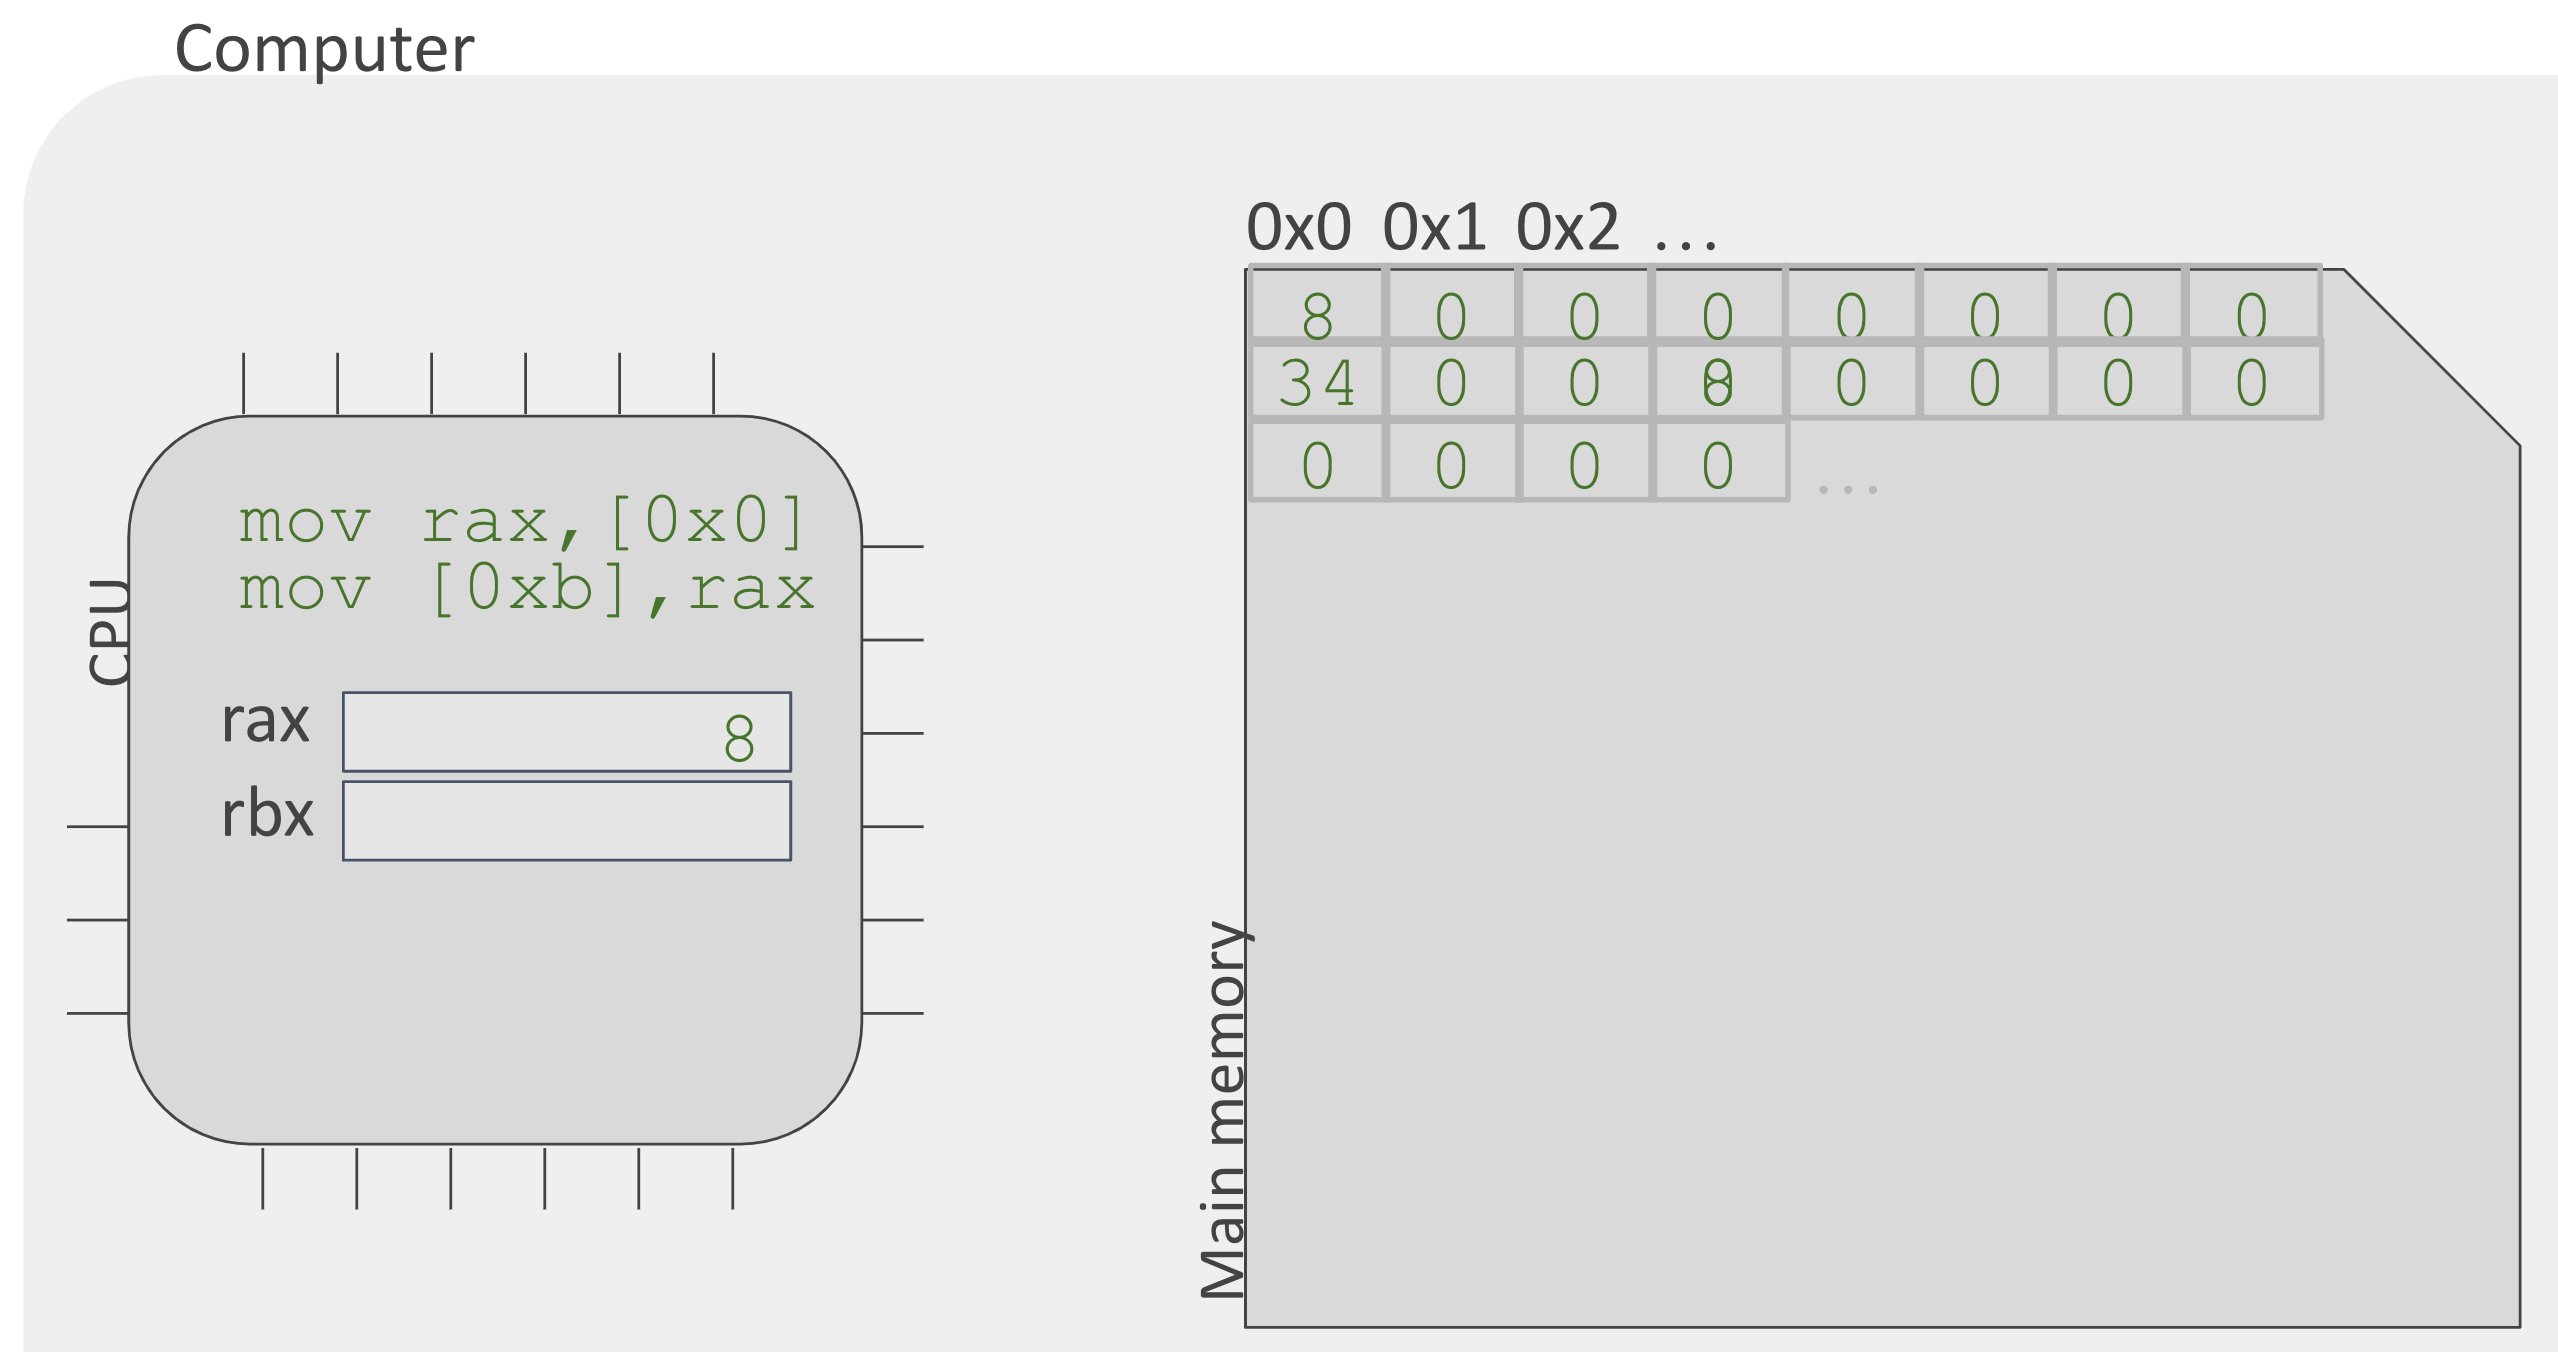
\includegraphics[width=0.45\textwidth]{chapters/L4/images/main-mem.png}
\end{center}
\newpage
\subsection{Instruction Pointer}
A key component in the CPU's control mechanism is the \emph{instruction pointer} (IP), in some contexts (ie. FDS, Comparch), this register is also known as the \emph{program counter} (PC), but the term "instruction pointer" more precisely describes its function.
\vspace{10px}
\begin{definition}[Instruction Pointer]
\leavevmode\\[5px]
The \textbf{instruction pointer} is a CPU register that holds the memory address of the next instruction to be executed.
\end{definition}
\vspace{5px}
\subsection{Subparts of Main Memory}
Main memory contains not only the memory images of individual processes but also the code and data essential to the operating system (OS). The OS comprises several critical components that ensure the proper operation and usability of the computer. These components include:

\begin{itemize}
  \item \textbf{Process Memory Images:} Every process has its own memory image, typically divided into:
  \begin{itemize}
    \item \textbf{Data Segment:} Stores global variables.
    \item \textbf{Stack Segment:} Contains local variables, return addresses, and other function call-related data.
    \item \textbf{Heap Segment:} Holds dynamically allocated memory (e.g., allocated via \texttt{malloc}).
  \end{itemize}
  \vspace{5px} 
  \item \textbf{Operating System Code:} This comprises all the code necessary for the computer's operation and usability. OS code is organized into:
    \begin{itemize}
      \item \emph{Kernel:} The central component of the OS, running in high-privilege mode. It manages system resources, hardware interactions, and security, ensuring the core functions of the computer operate correctly. It is neither a process nor a library (end of lecture explains).
        \begin{itemize}
          \item It creates and deletes processes and threads.
          \item It initiates I/O.
          \item It handles errors and interrupts.
          \item It decides which thread will run next.
        \end{itemize}
      \item \emph{Processes:} Such as the graphical user interface (GUI) and terminal applications, which provide user-level interaction with the system.
      \item \emph{Libraries:} Modules like the standard C library that provide a suite of functions, which are dynamically integrated into processes when called.
    \end{itemize}
\end{itemize}

\begin{center}
  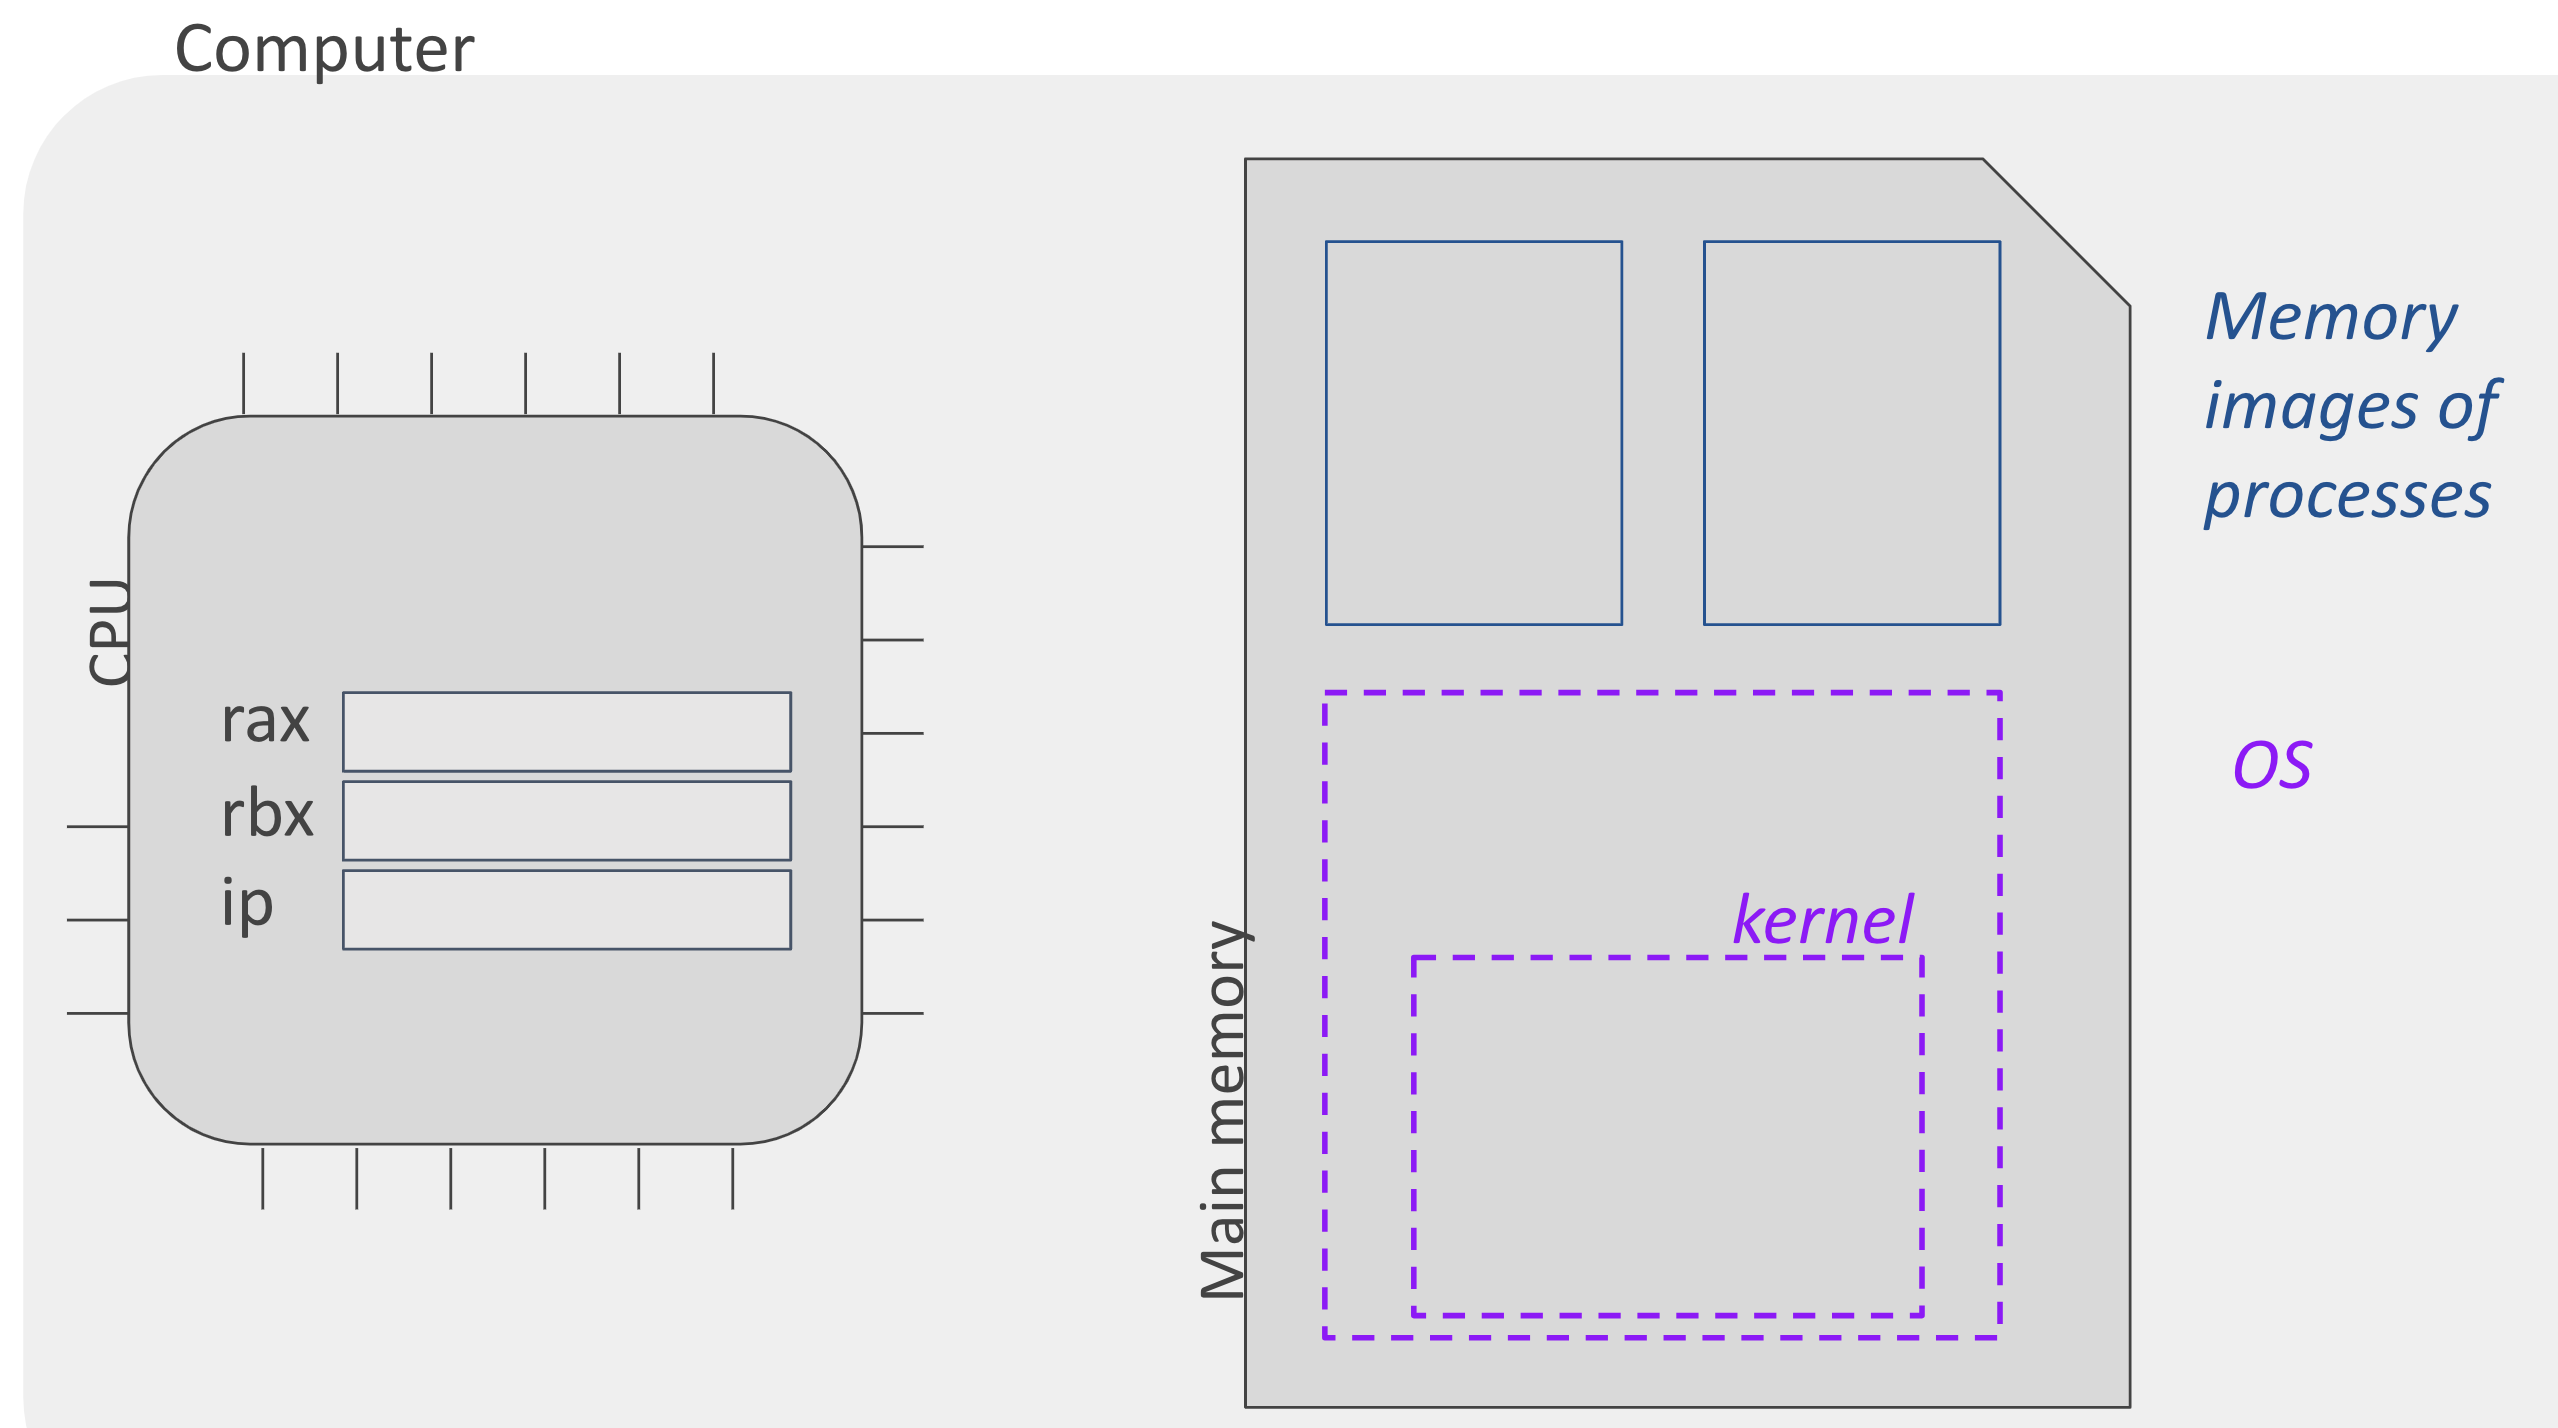
\includegraphics[width=0.45\textwidth]{chapters/L4/images/main-mem-content.png}
\end{center}
\newpage
\section{Process Memory Image}
\begin{definition}[Process Memory Image]
  \leavevmode\\[5px]
A \textbf{process memory image} is the complete layout of a process's memory, comprising:
\begin{itemize}
  \item[-] The \emph{text segment} for the process's code.
  \item[-] The \emph{data segment} for global variables.
  \item[-] The \emph{stack segment} for local variables and return pointers.
  \item[-] The \emph{heap segment} for dynamically allocated memory. (eg. malloc)
\end{itemize}
\end{definition}

\vspace{10px}
\noindent
\begin{minipage}{0.45\textwidth}
  \textbf{Exam Question:} We provide you with a C program. Your task is to draw the memory image of the corresponding process at different points in the program.
\begin{enumerate}
    \item Mark each segment, even if it is empty.
    \item Draw a schema of the code in the \textbf{Text Segment}, including only function names and calls in assembly.
    \item Identify global variables and place them in the \textbf{Data Segment} (e.g., \texttt{g:0}).
    \item Simulate each step of the program’s execution to fill the \textbf{Heap} and \textbf{Stack} segments accordingly. This includes local variables, memory allocations, and function calls.
\end{enumerate}
\end{minipage}
\hfill
\vline
\hfill
\begin{minipage}{0.45\textwidth}
    \begin{center}
    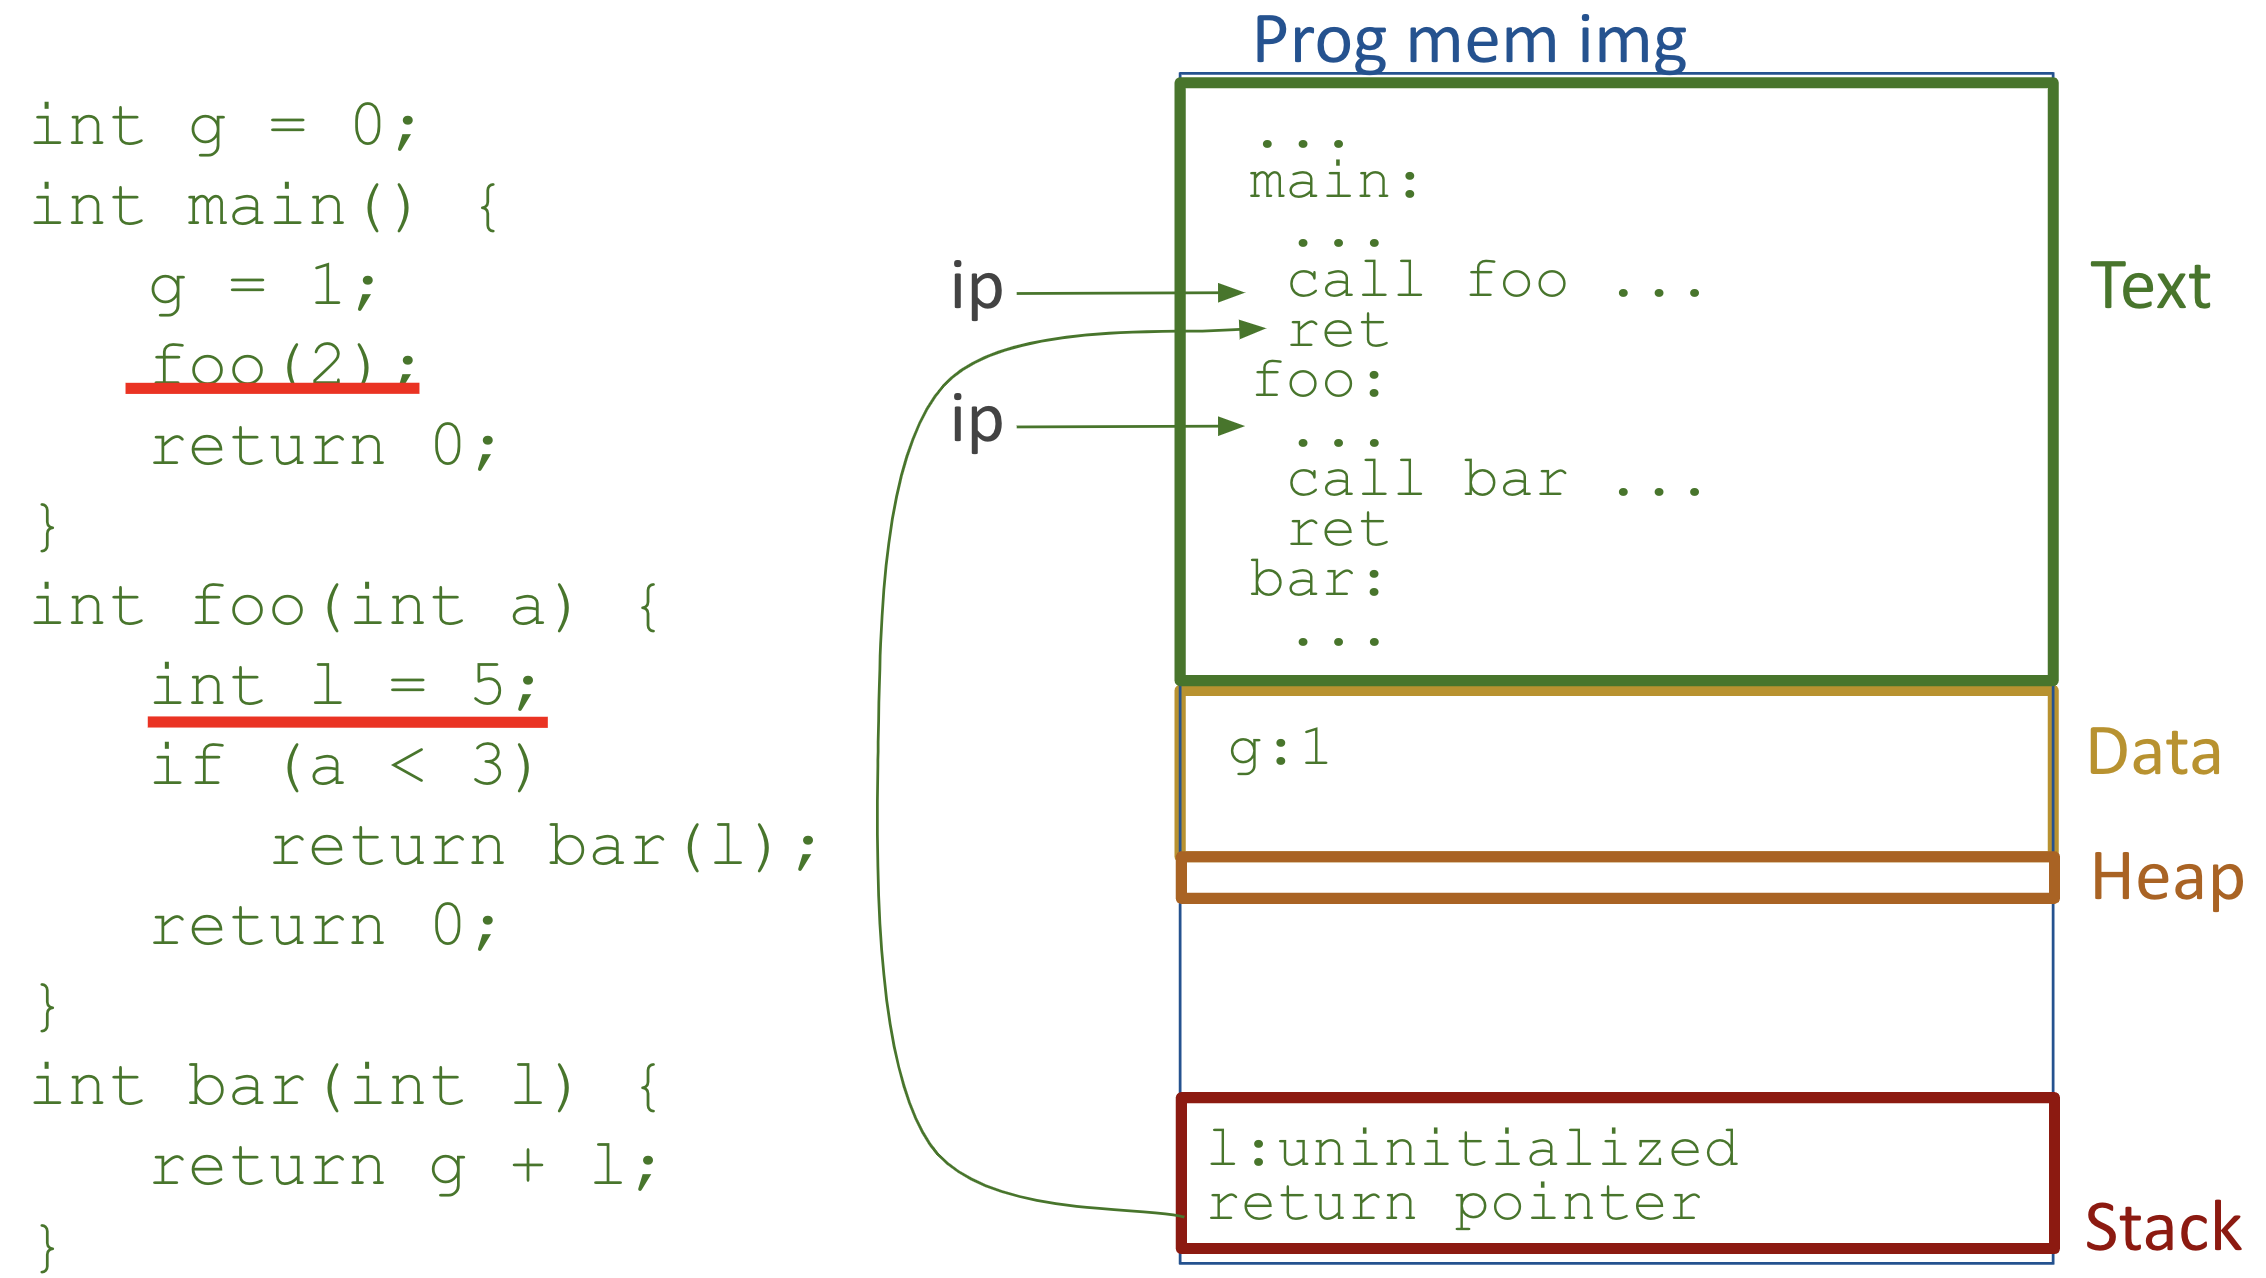
\includegraphics[width=1.23\textwidth]{chapters/L4/images/exam.png}
\end{center}
\end{minipage} \\[30px]

\textbf{Exam Question:} Show the memory image and indicate the moment when the stack reaches its maximum size.


For the program shown above, the expected result would be:
\begin{center}
  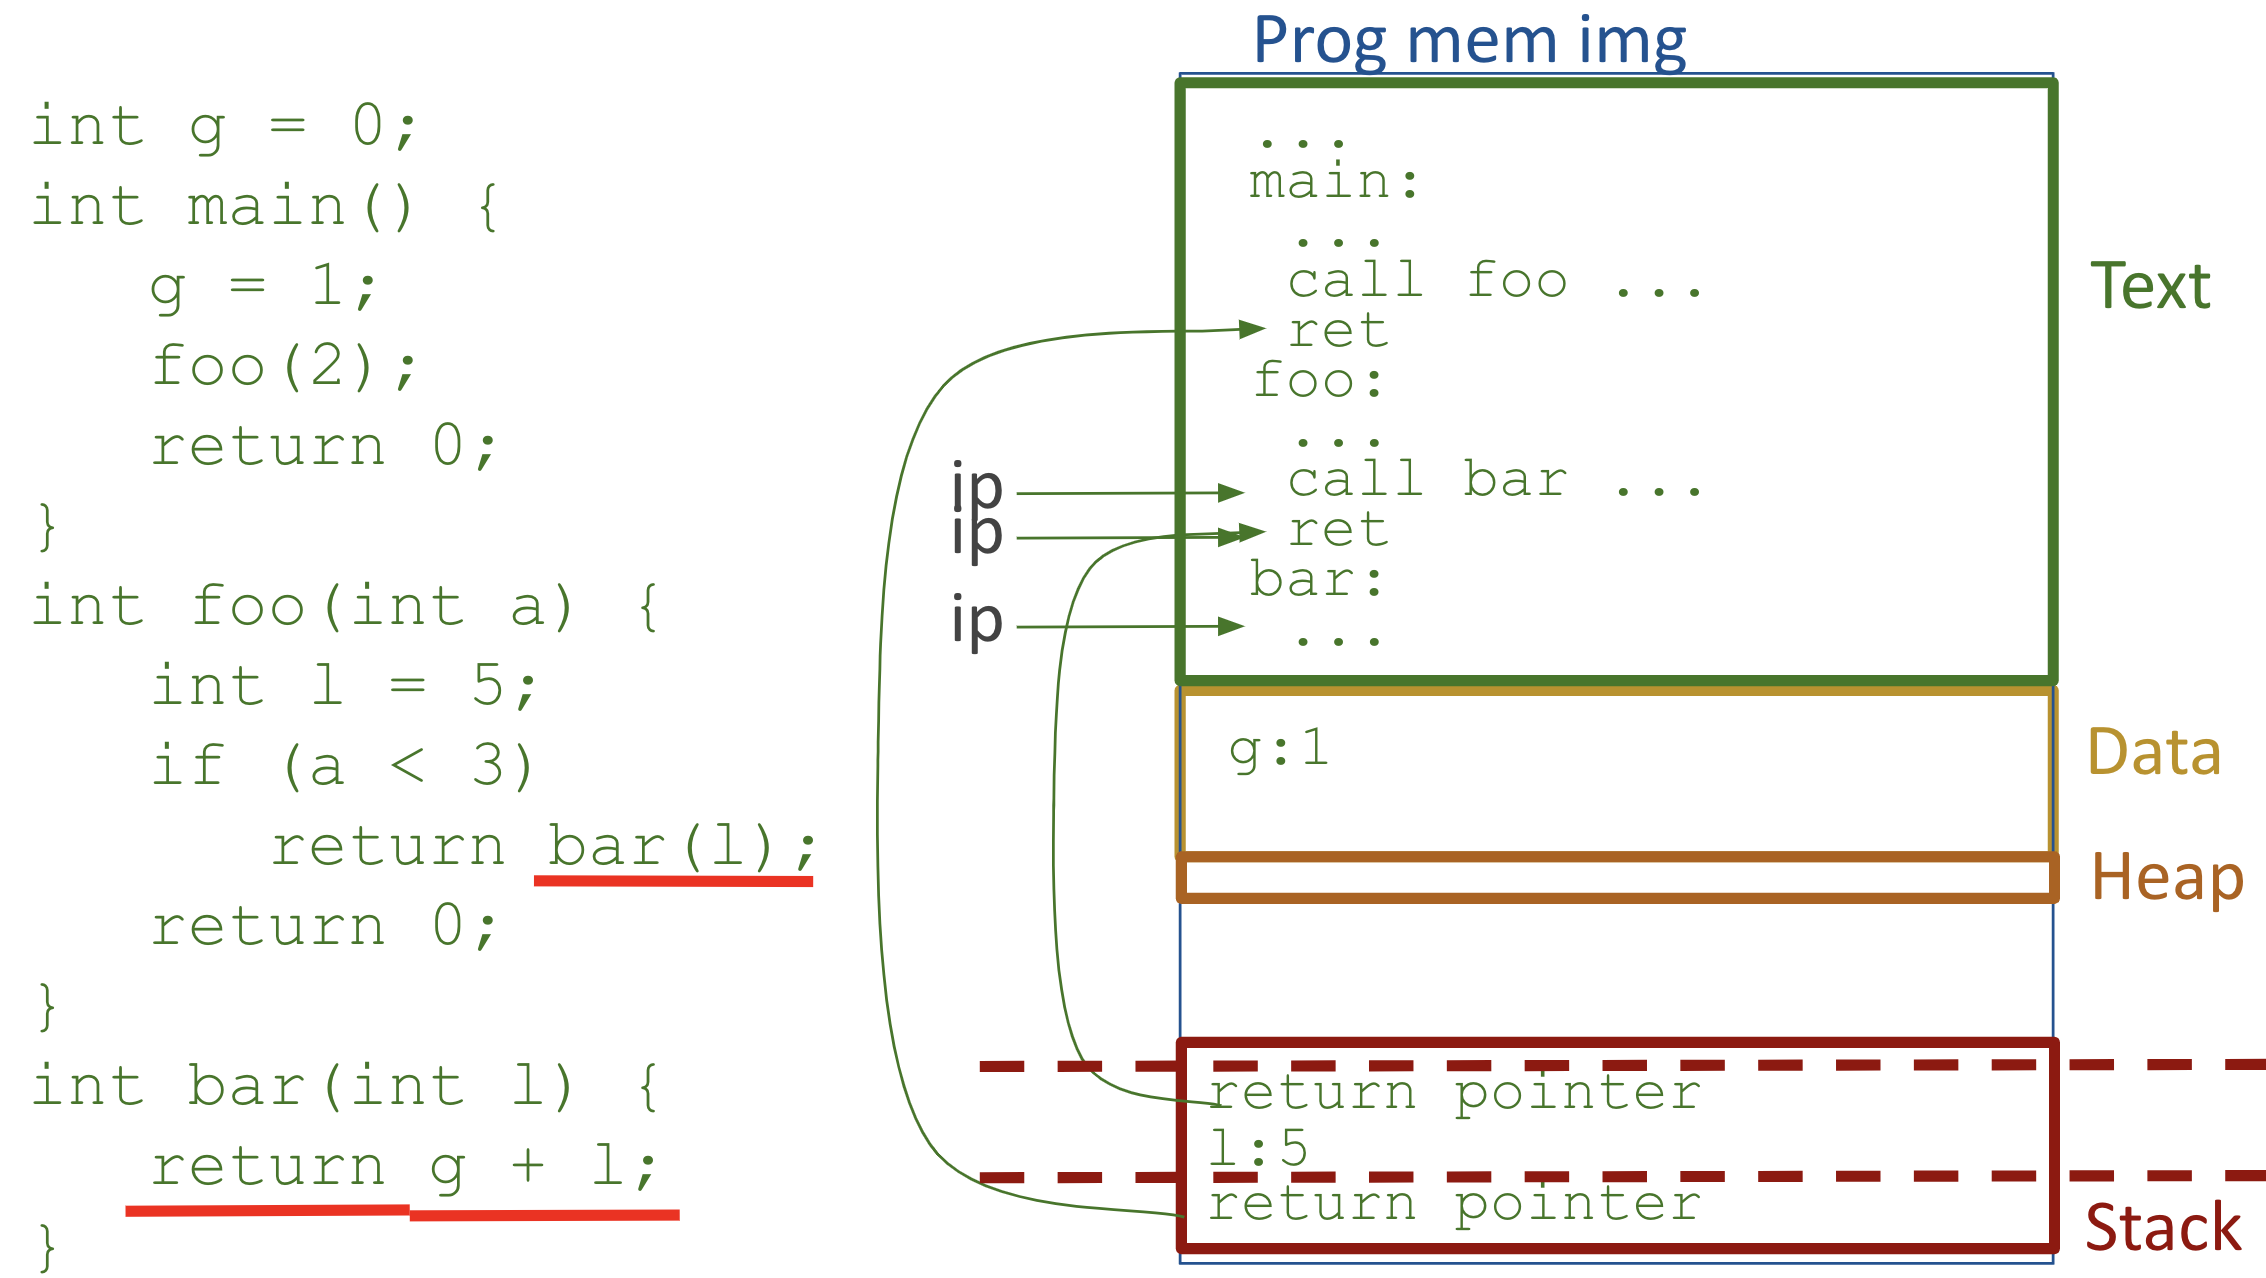
\includegraphics[width=0.65\textwidth]{chapters/L4/images/biggest-stack.png}
\end{center}

\newpage

\subsection{Optional - Stack and Register Functioning}

In modern computer architectures, the process of a function call involves a coordinated interplay between CPU registers and the stack.\\[8px]

\begin{definition}[Function Call Mechanism]
\leavevmode\\[5px]
During a function call:
\begin{enumerate}
    \item The \textbf{caller} passes arguments to the \textbf{callee} by storing values in designated CPU registers.
    \item The \textbf{callee} processes the call and returns a result by placing it in a specific register (for example, the \texttt{rax} register).
\end{enumerate}
\end{definition}

\begin{center}
    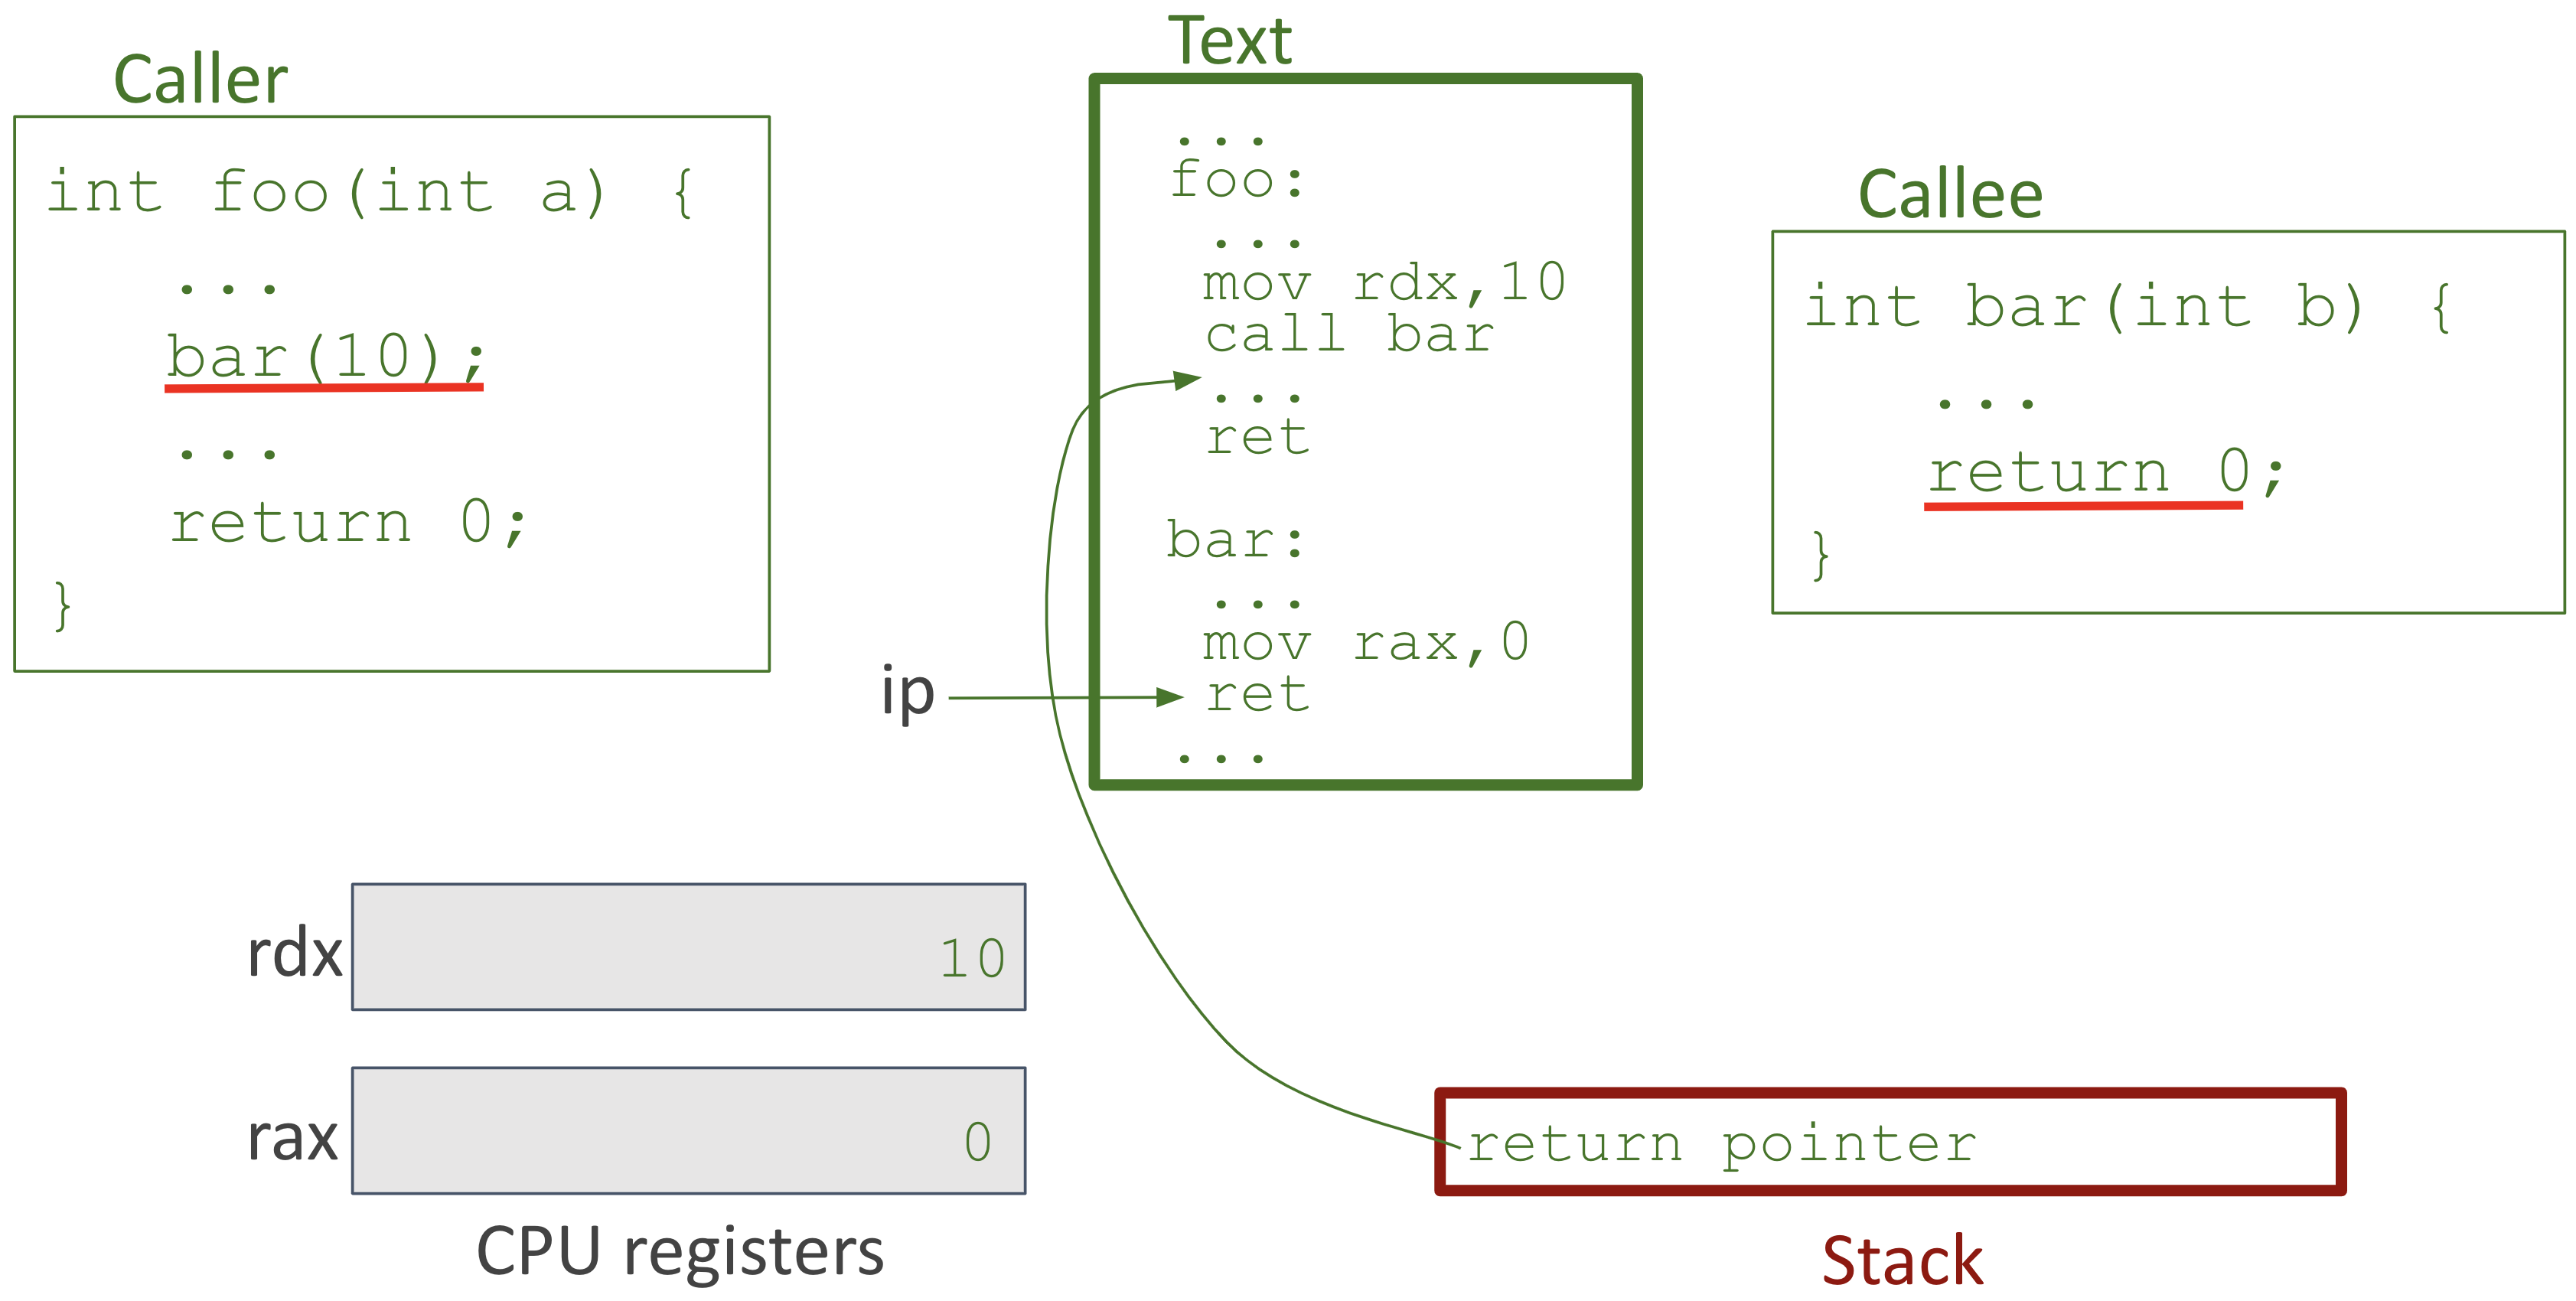
\includegraphics[width=0.65\textwidth]{chapters/L4/images/foo-bar.png}
\end{center}
\vspace{10px}
\begin{example}[Illustrative Function Call]
Consider the scenario where function \texttt{Foo} calls function \texttt{Bar}:
\begin{enumerate}
    \item \textbf{Argument Passing:} \texttt{Foo} stores the argument value (e.g., \textbf{10}) in a CPU register. 
    \item \textbf{Return Value Handling:} An implicit agreement between foo and bar that the return value will be stored in a particular register (eg. rax). \texttt{Bar} processes the argument and stores its return value in another register (e.g., \texttt{rax}). Later, \texttt{Foo} retrieves this value by accessing that register.
\end{enumerate}
\end{example}

A caller and a callee share common infrastructure by using CPU registers to maintain their context during the call. In addition, the stack is used to preserve register states when necessary:
\begin{itemize}
    \item \textbf{Caller-Saved Registers:} The caller saves certain registers to the stack before the call and restores them after the call returns.
    \item \textbf{Callee-Saved Registers:} The callee saves its registers at the beginning of the function and restores them before returning.
\end{itemize}
\textit{The stack, the register the calling conventions form a caller/callee interface.}\\
Adhering to these calling conventions is critical; for instance, if the callee writes into the caller's stack frame, it may lead to stack smashing and compromise program stability.



\newpage
\section{Memory Virtualization}
In modern operating systems, each process references memory using virtual addresses. Underneath, these virtual addresses are translated to physical addresses. Importantly, each process has its own virtual address space, which means that two processes may use the same virtual address while referring to entirely different physical locations. This design creates the \textbf{safe illusion} that main memory “belongs” exclusively to each process, greatly simplifying program development and enhancing security.

\noindent
\begin{minipage}{0.45\textwidth}
Each address in the image refers to an address within its own stack. The addresses shown are \emph{virtual}, meaning they are process-specific (e.g., address 0 in one process does not necessarily correspond to address 0 in another).
\end{minipage}%
\hfill
\vline
\hfill
\begin{minipage}{0.45\textwidth}
\begin{center}
    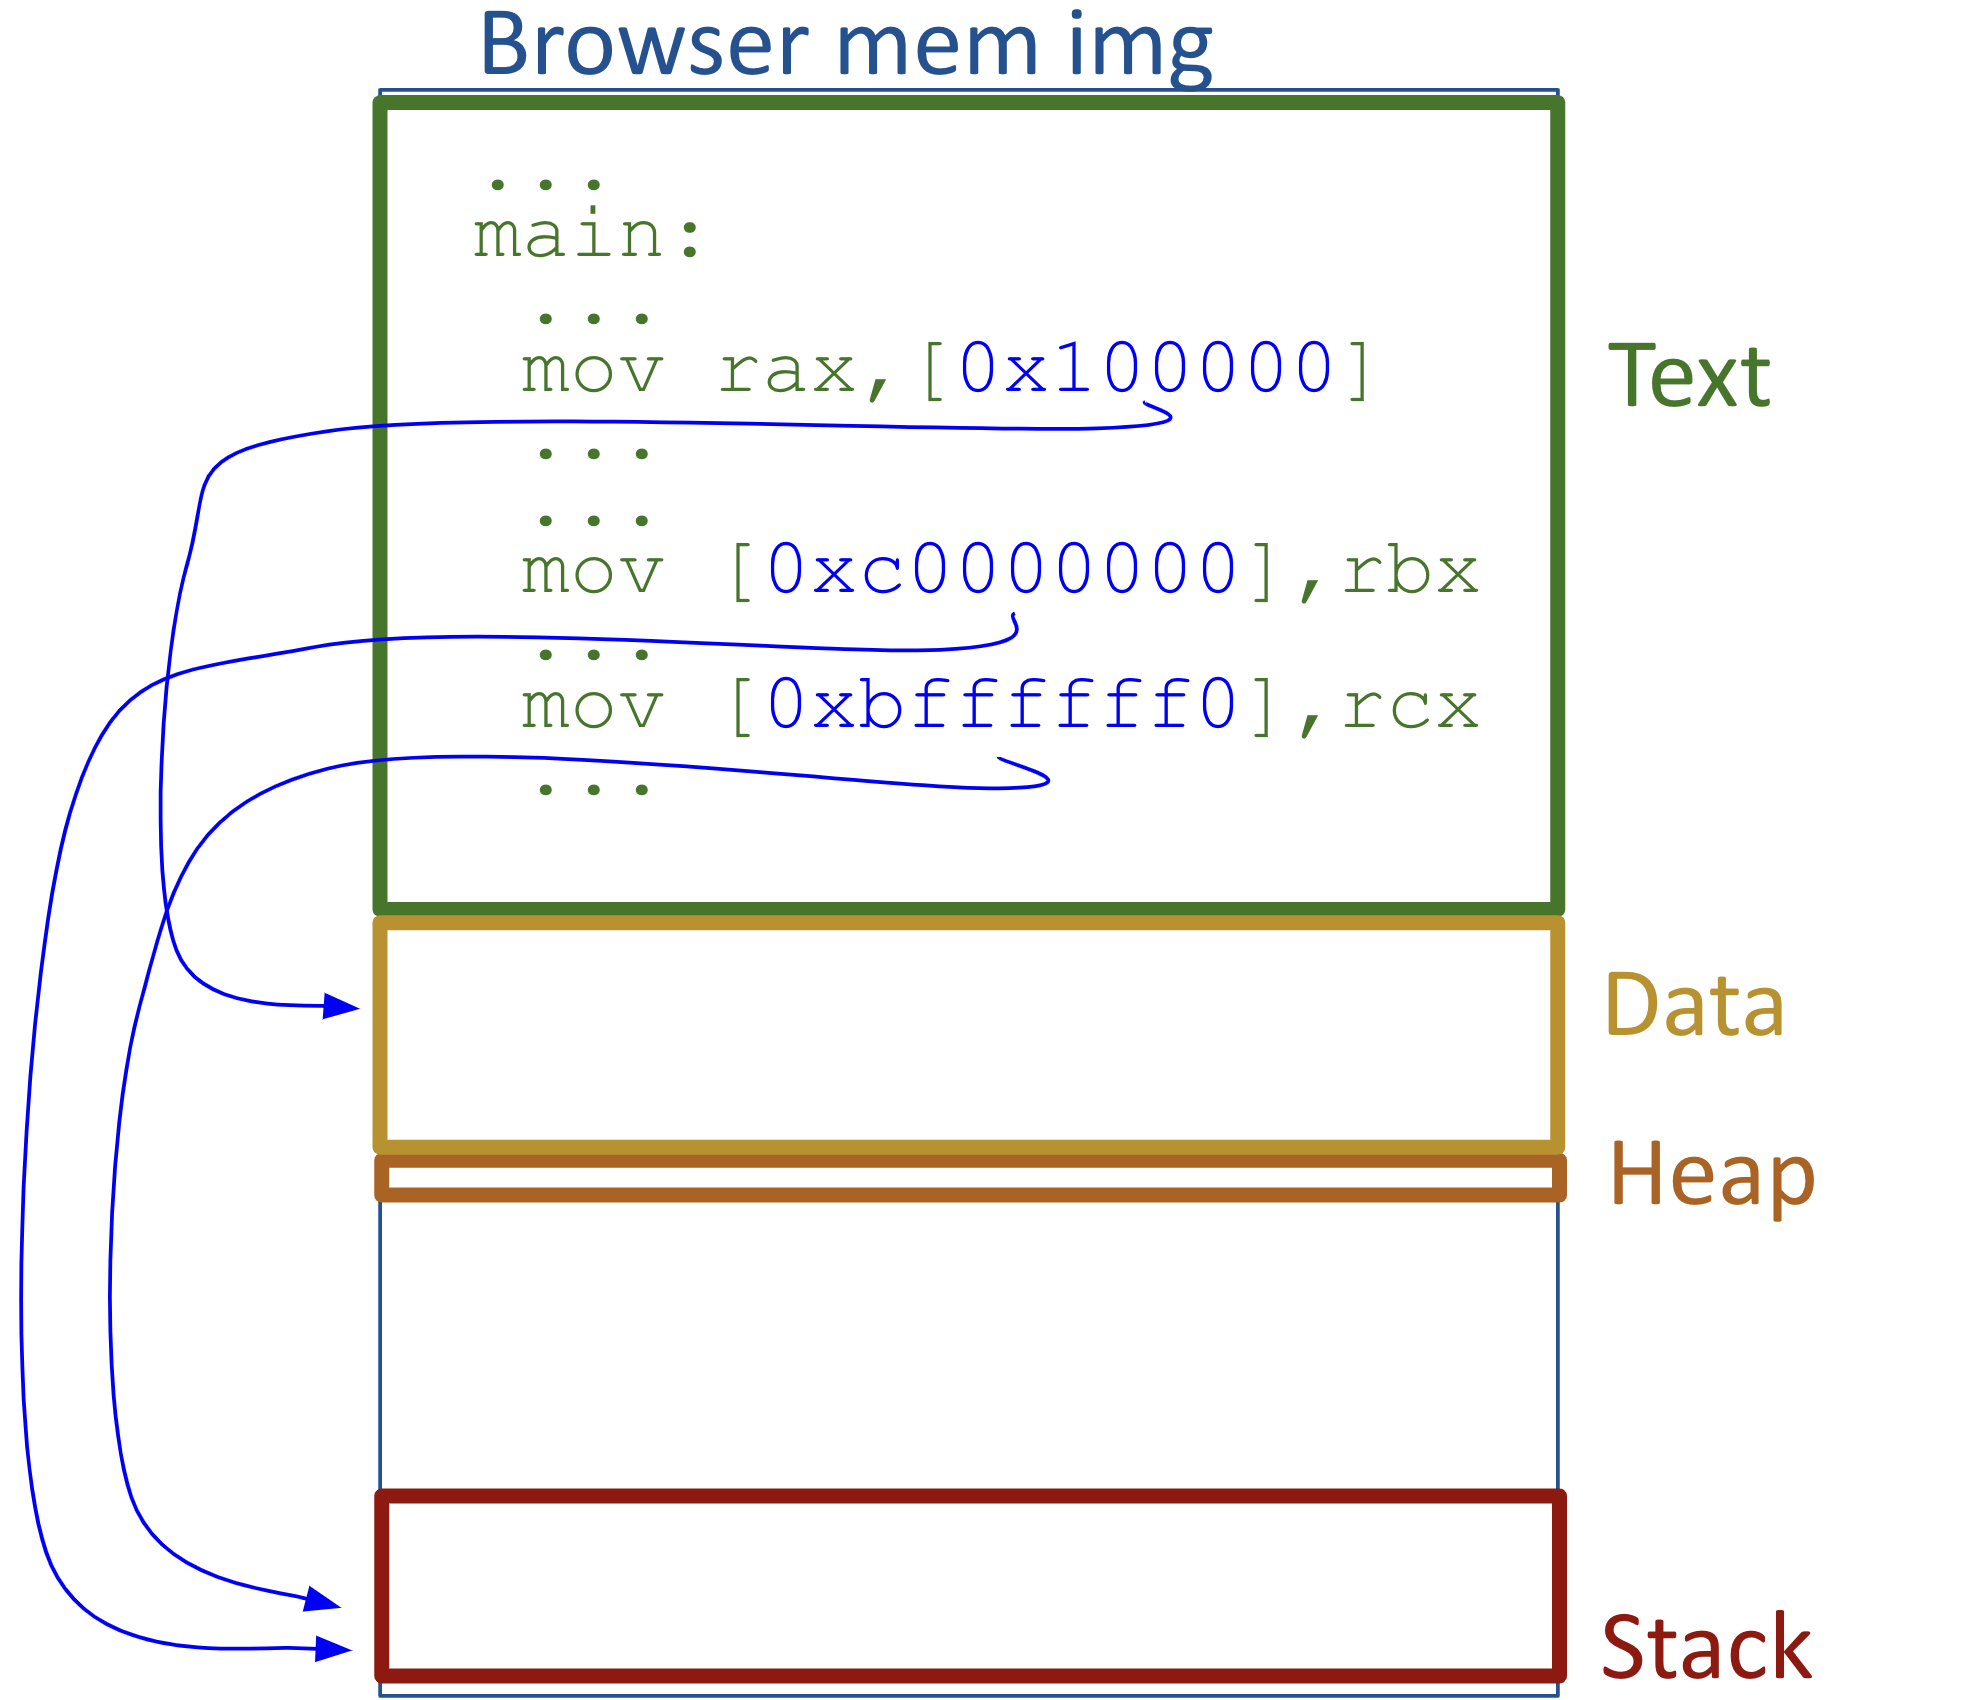
\includegraphics[width=0.85\textwidth]{chapters/L4/images/browser-img.png}
\end{center}
\end{minipage}\\[10px]

\noindent
\begin{minipage}{0.45\textwidth}
\textbf{Exam Question:} If two memory instructions read the same virtual address, is it the same physical address? \\[3px]
\textbf{Answer:} Yes, when they are translated to the same physical memory address, as they belong to the same virtual address space.
\end{minipage}%
\hfill
\vline
\hfill
\begin{minipage}{0.45\textwidth}
\begin{center}
    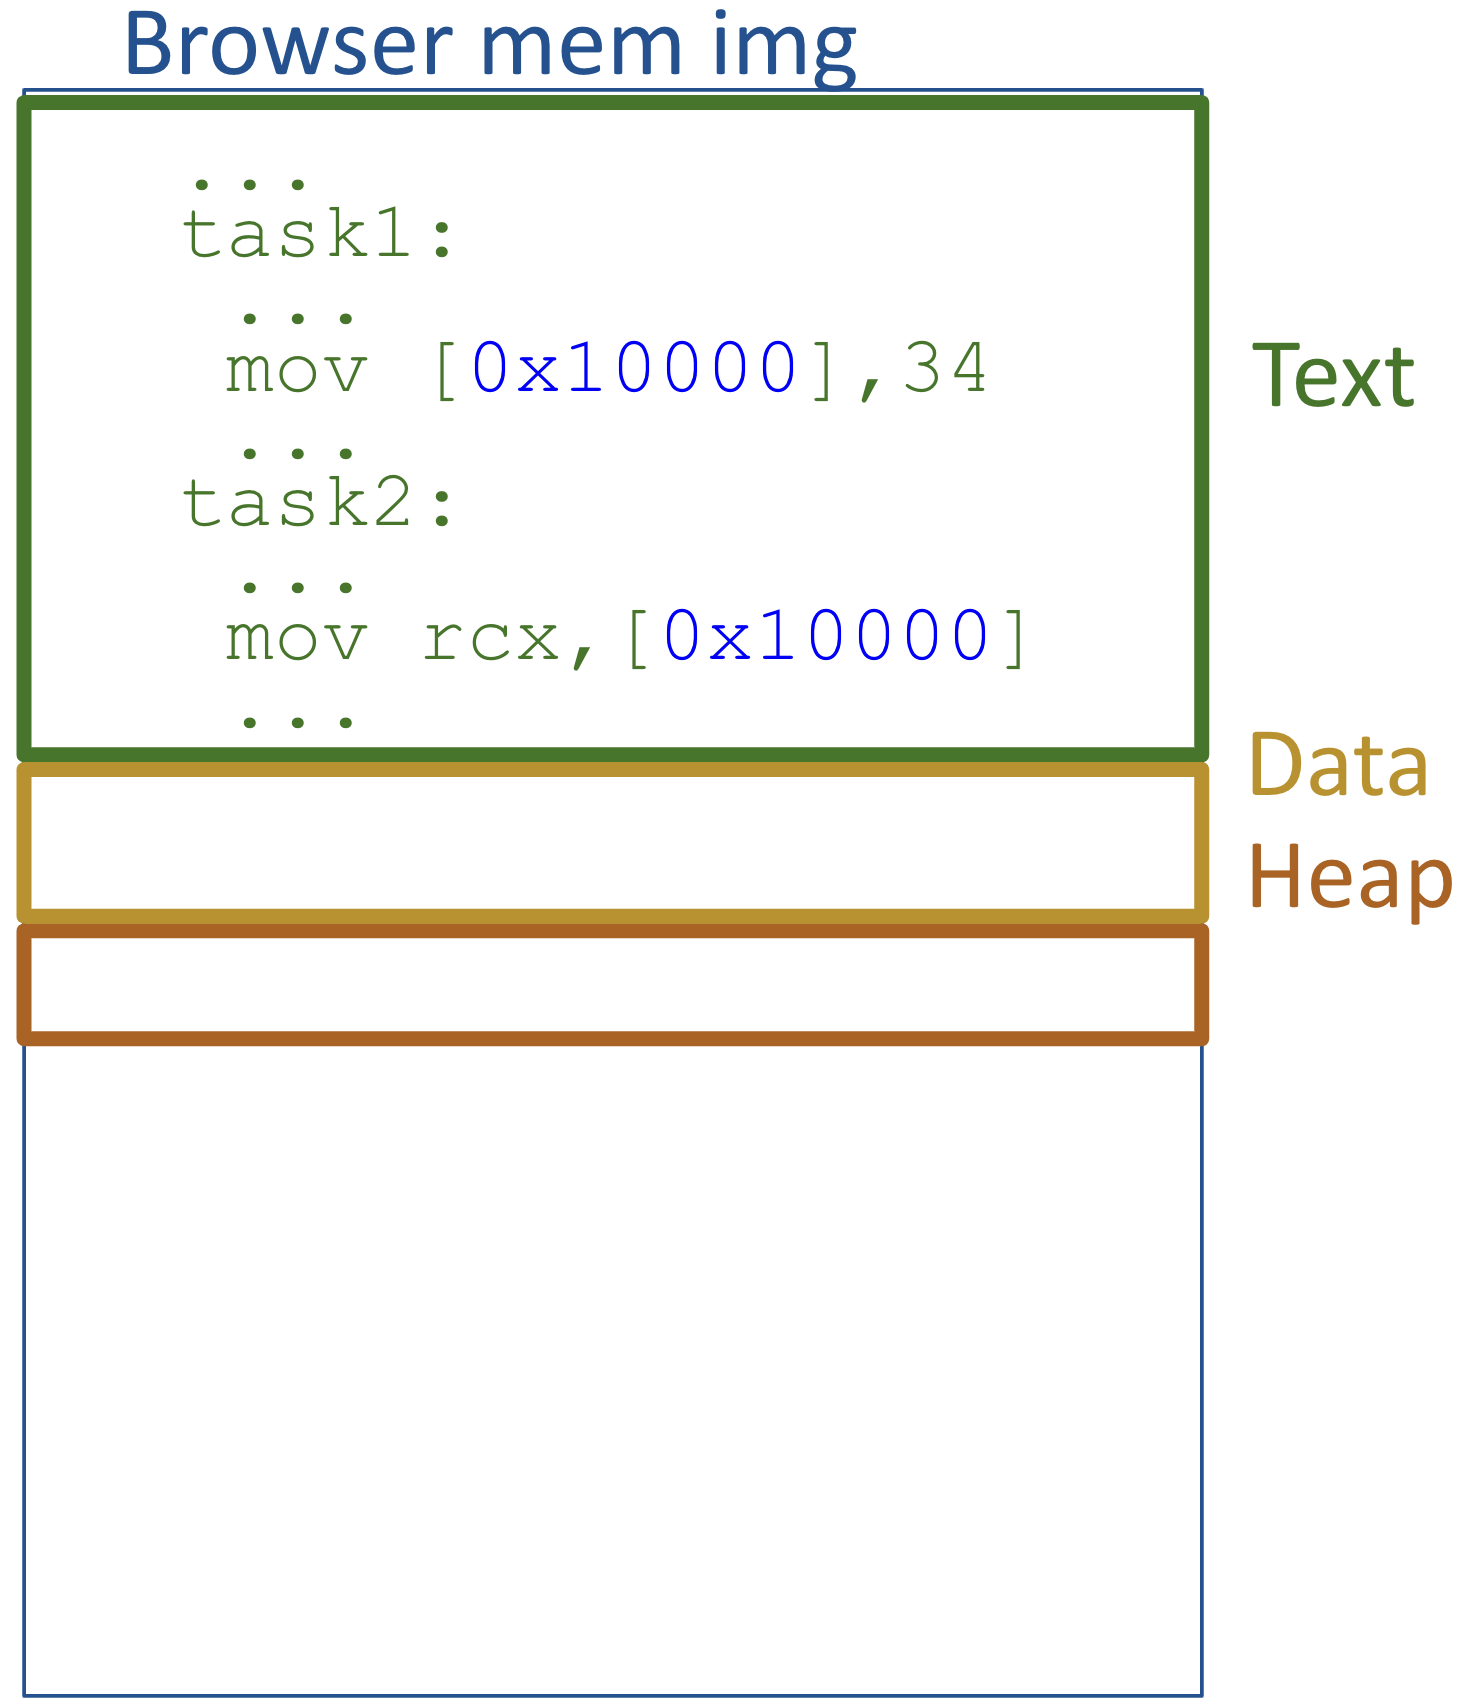
\includegraphics[width=0.7\textwidth]{chapters/L4/images/two-proc.png}
\end{center}
\end{minipage}
\\[10px]

\noindent
\begin{minipage}{0.45\textwidth}
\textbf{Exam Question:} Are these two processes accessing the same memory location? \\[3px]
\textbf{Answer:} No, they are not actually accessing the same physical memory. Although both use the address 0x10000, each process runs in its own virtual address space. 
\end{minipage}%
\hfill
\vline
\hfill
\begin{minipage}{0.45\textwidth}
\begin{center}
    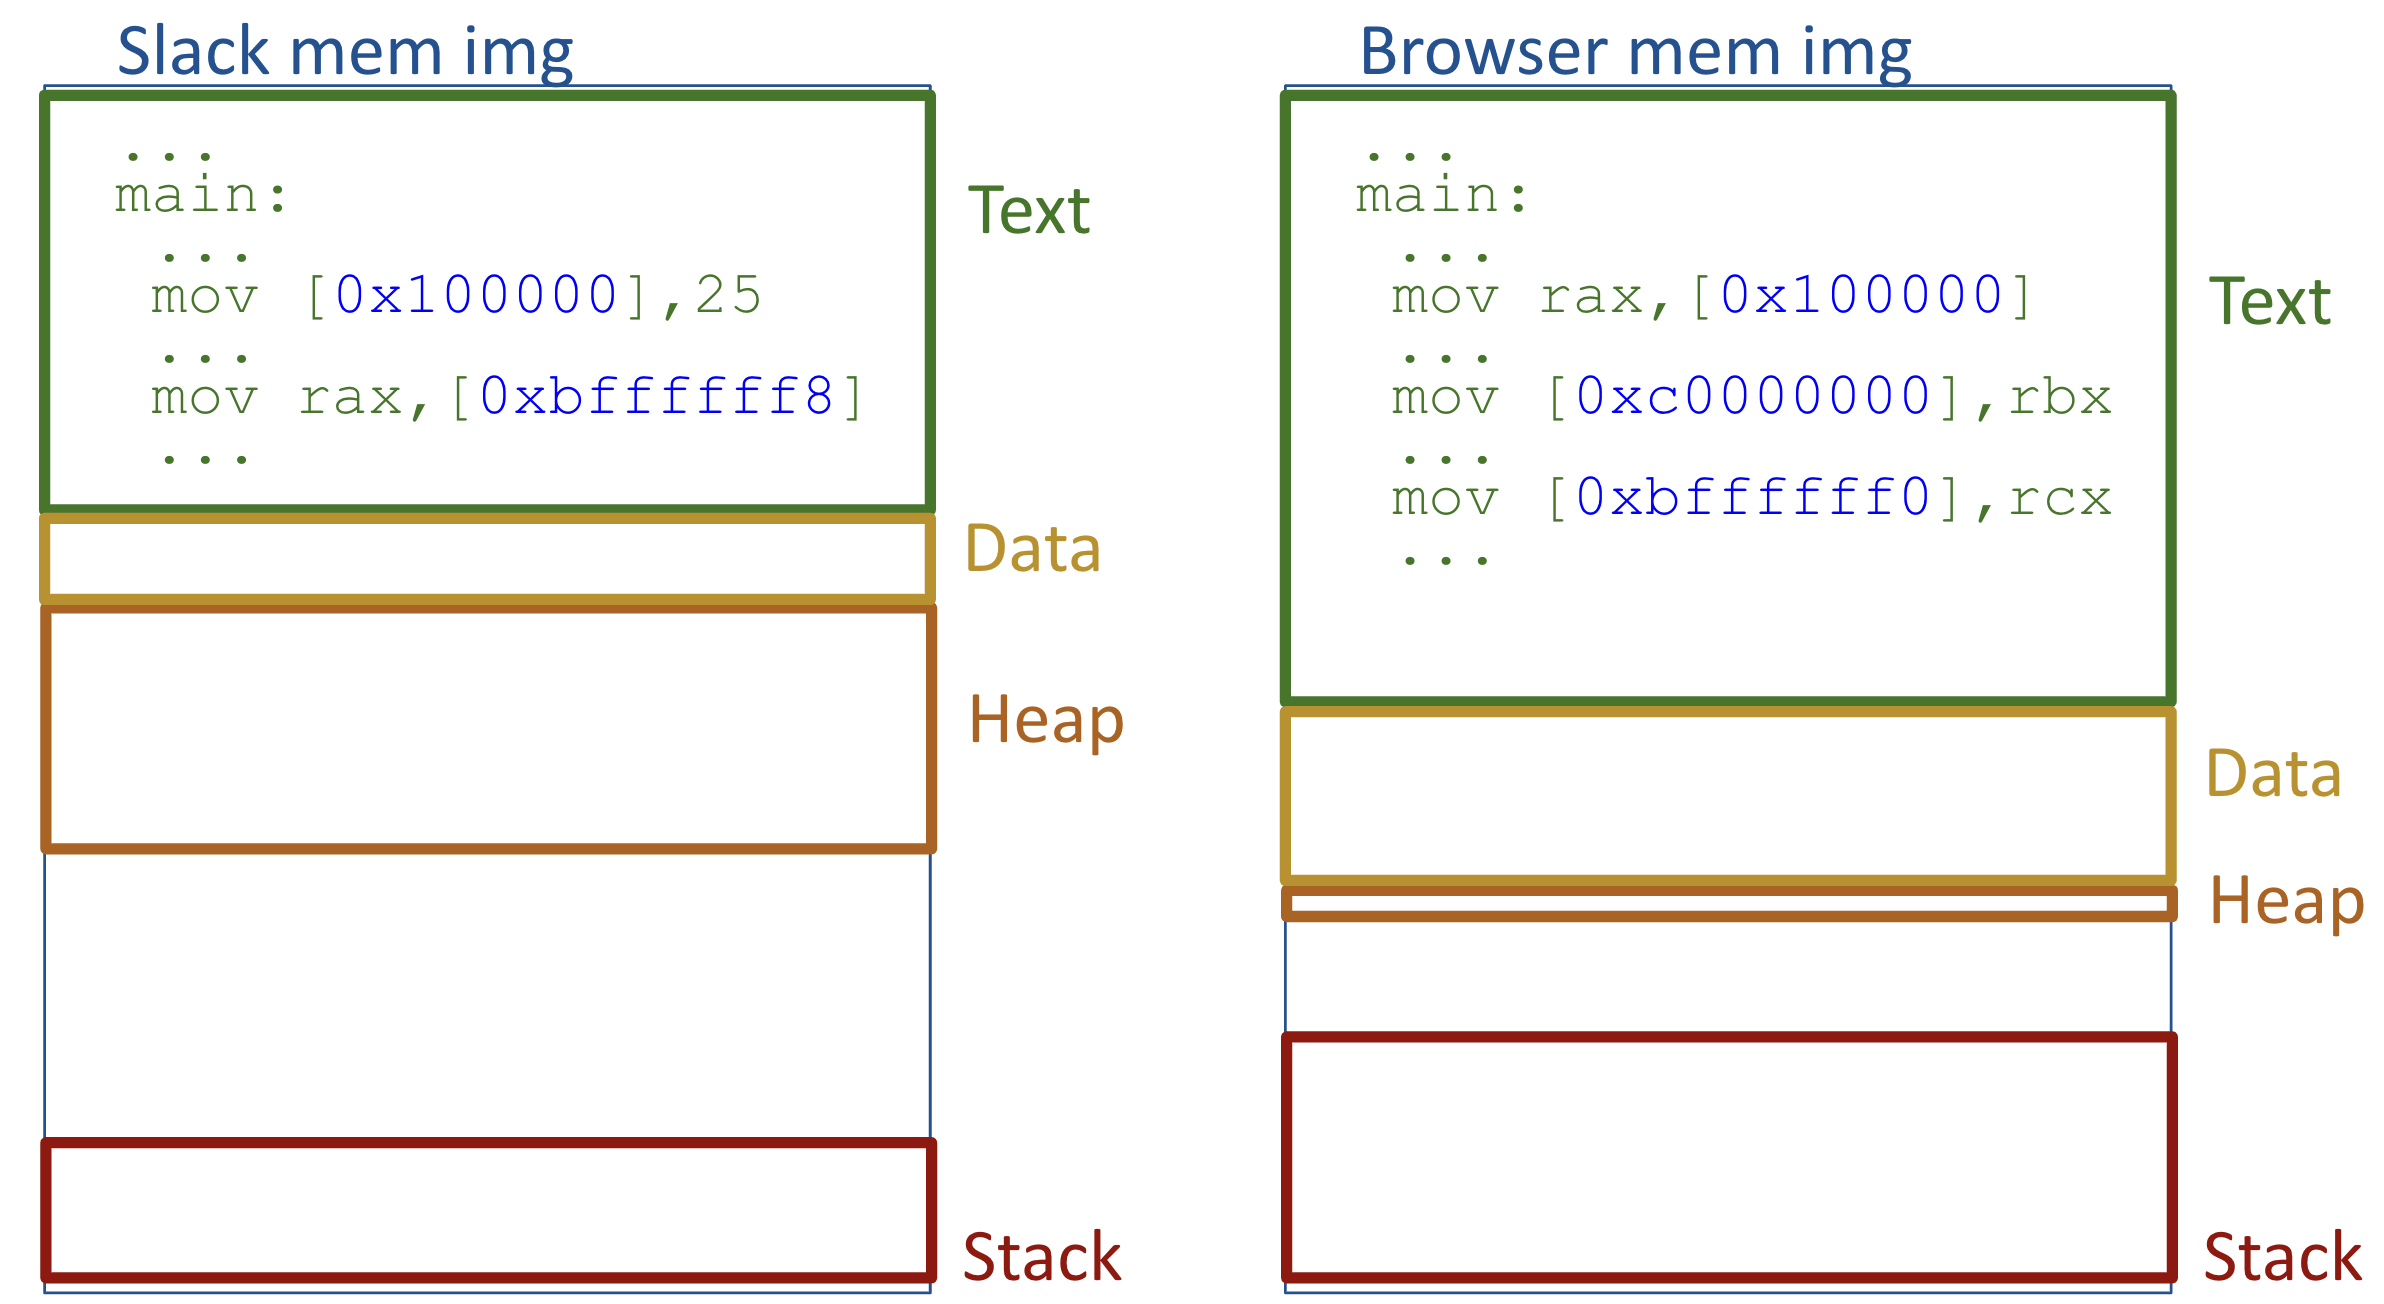
\includegraphics[width=1.25\textwidth]{chapters/L4/images/virtual.png}
\end{center}
\end{minipage}\\[14px]

The mechanism of memory virtualization creates a \emph{safe illusion} in which it appears that the main memory is exclusively owned by each process. This design not only simplifies the generation of executable programs but also enforces security by ensuring that a process can only access its own memory image.

\begin{definition}[Contiguous Memory]
\leavevmode\\[2px]
Contiguous memory refers to a block of physical memory addresses that are sequentially arranged. In this allocation scheme, the entire memory image of a process is stored in one unbroken segment, simplifying the translation from virtual to physical addresses.
\end{definition}

\subsection{Memory Management Unit --- Simple Implementation}
\vspace{10px}
\noindent The \textbf{Memory Management Unit (MMU)} is a specialized piece of \textit{hardware} that translates virtual memory addresses into physical addresses.\\[10px]
\vspace{10px}
\noindent
\begin{minipage}{0.45\textwidth}
  For each process, the \textbf{OS kernel} sets up \emph{base} and \emph{bound} registers (which are physically stored in the CPU). The MMU then uses these values to ensure that the process’s memory image is allocated in a contiguous block of physical memory.\\[10px]
\begin{center}
  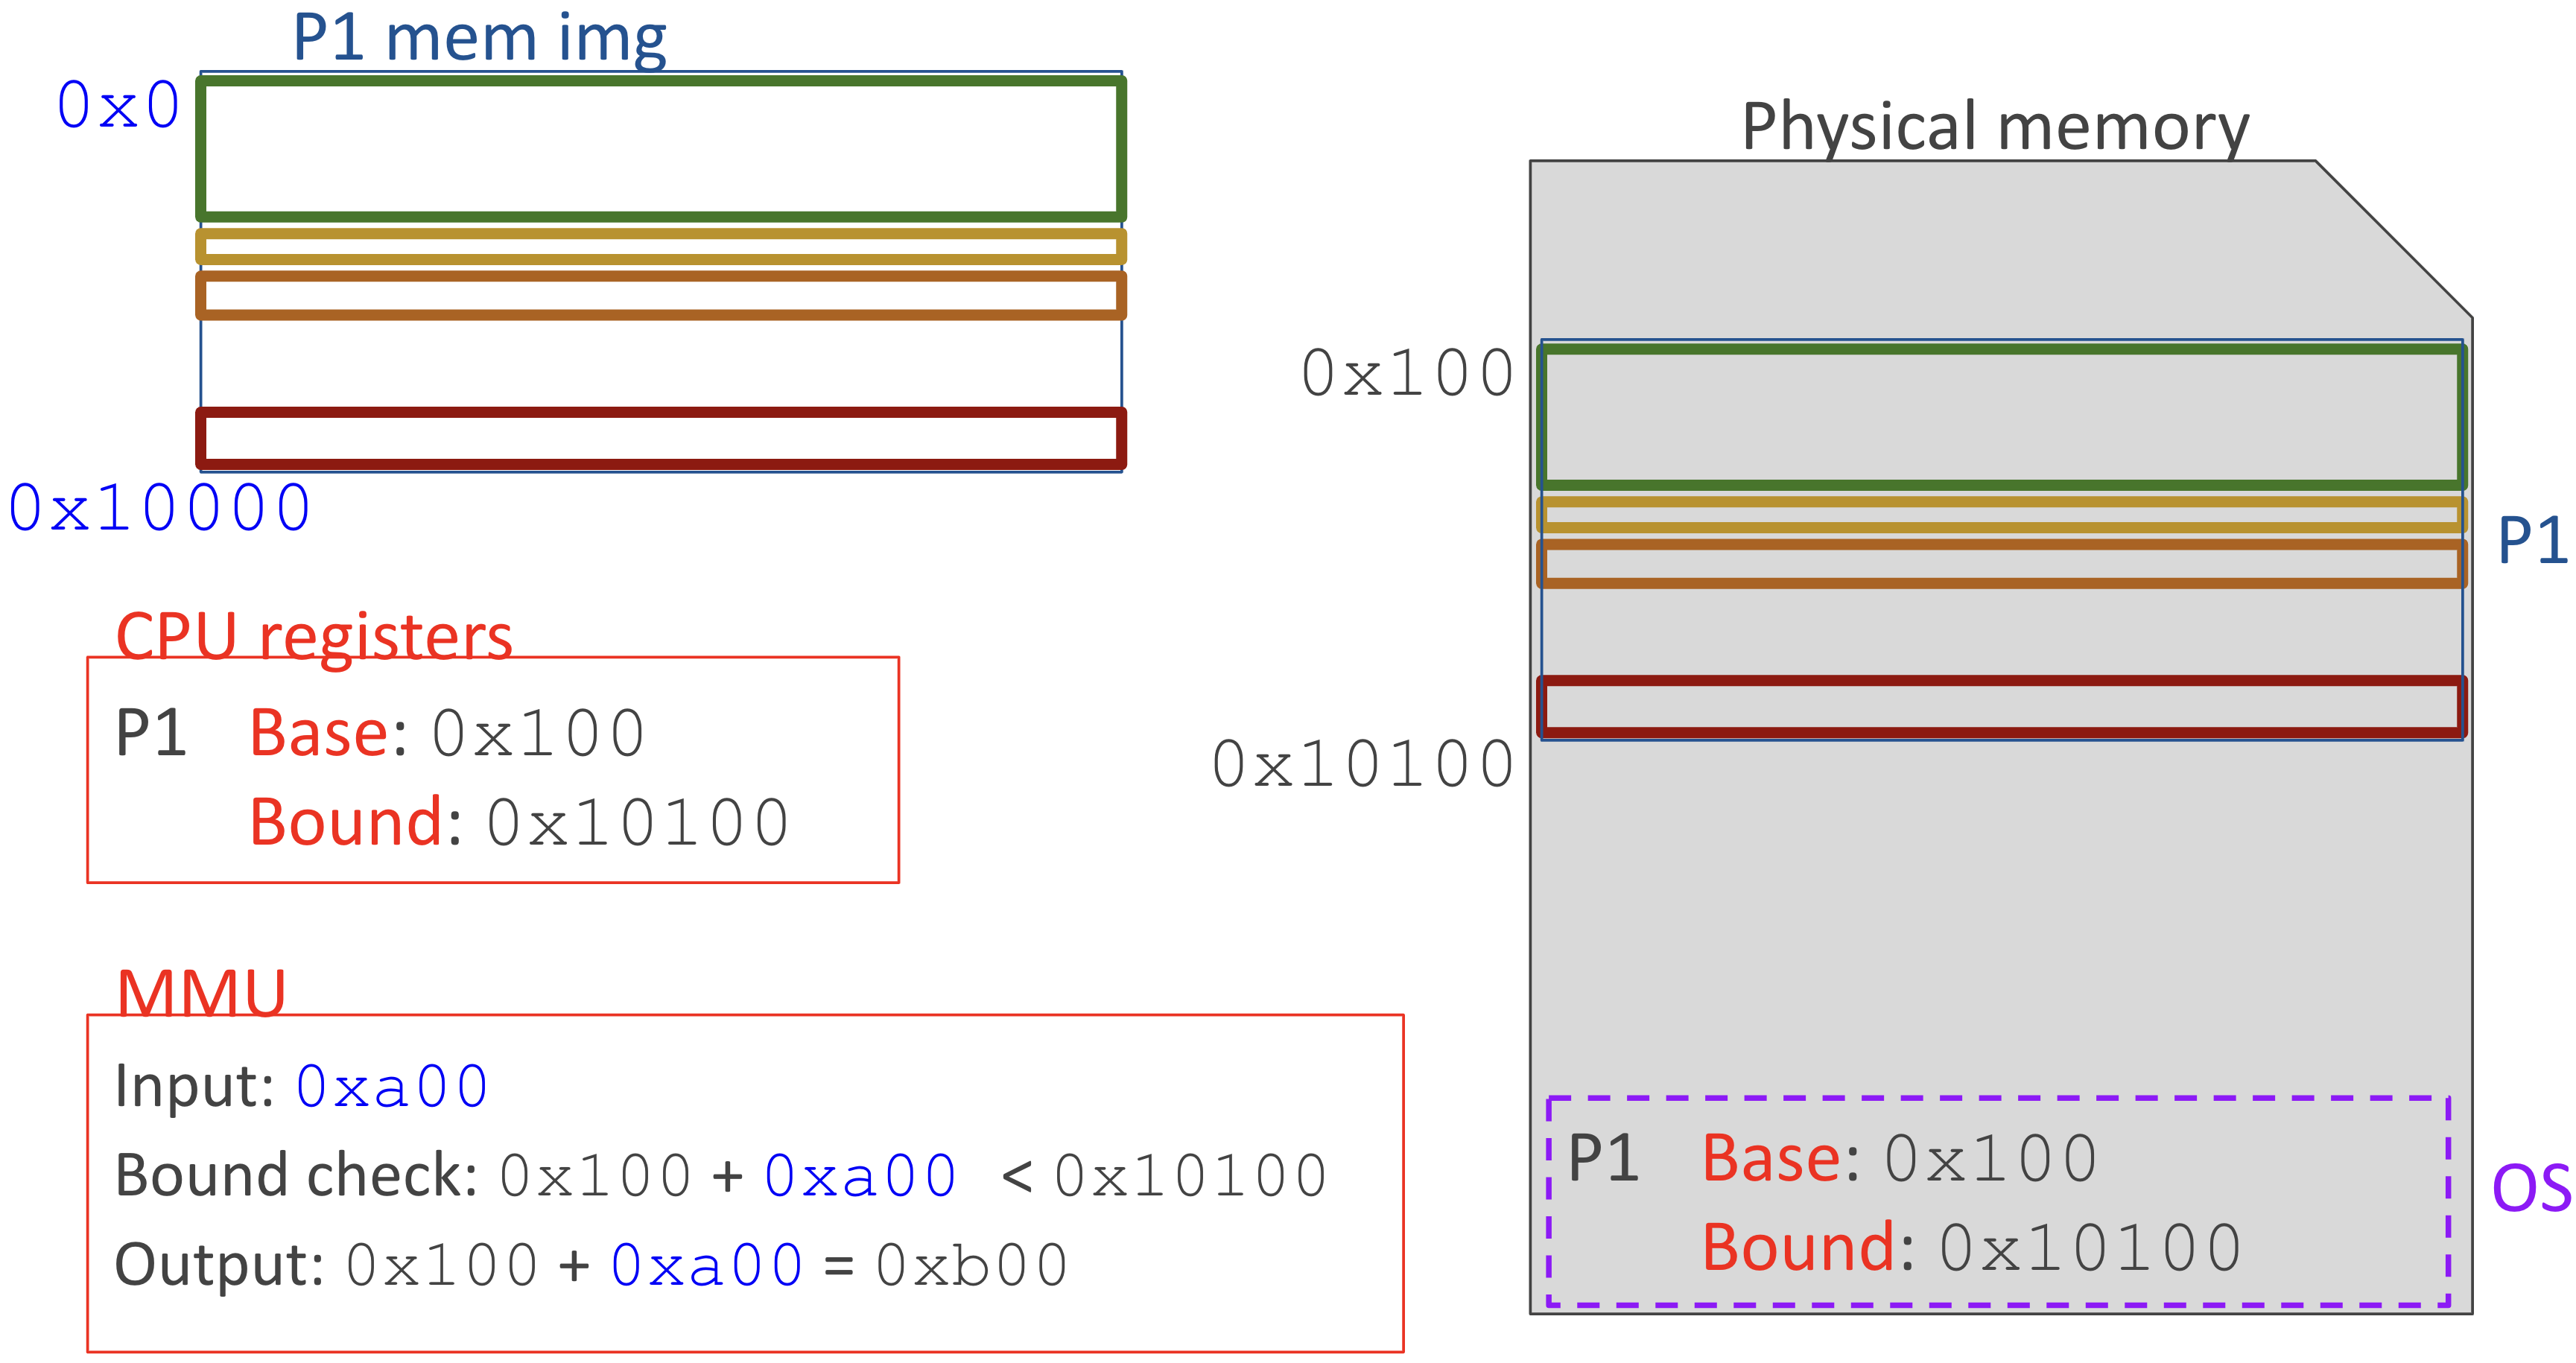
\includegraphics[width=1.1\textwidth]{chapters/L4/images/indirection.png}
\end{center}
\end{minipage}%
\hfill
\vline
\hfill
\begin{minipage}{0.45\textwidth}
\noindent When a second process (\(P_2\)) is introduced, the MMU checks its corresponding base and bound registers to determine the physical memory range in which \(P_2\) should be placed.
\begin{center}
  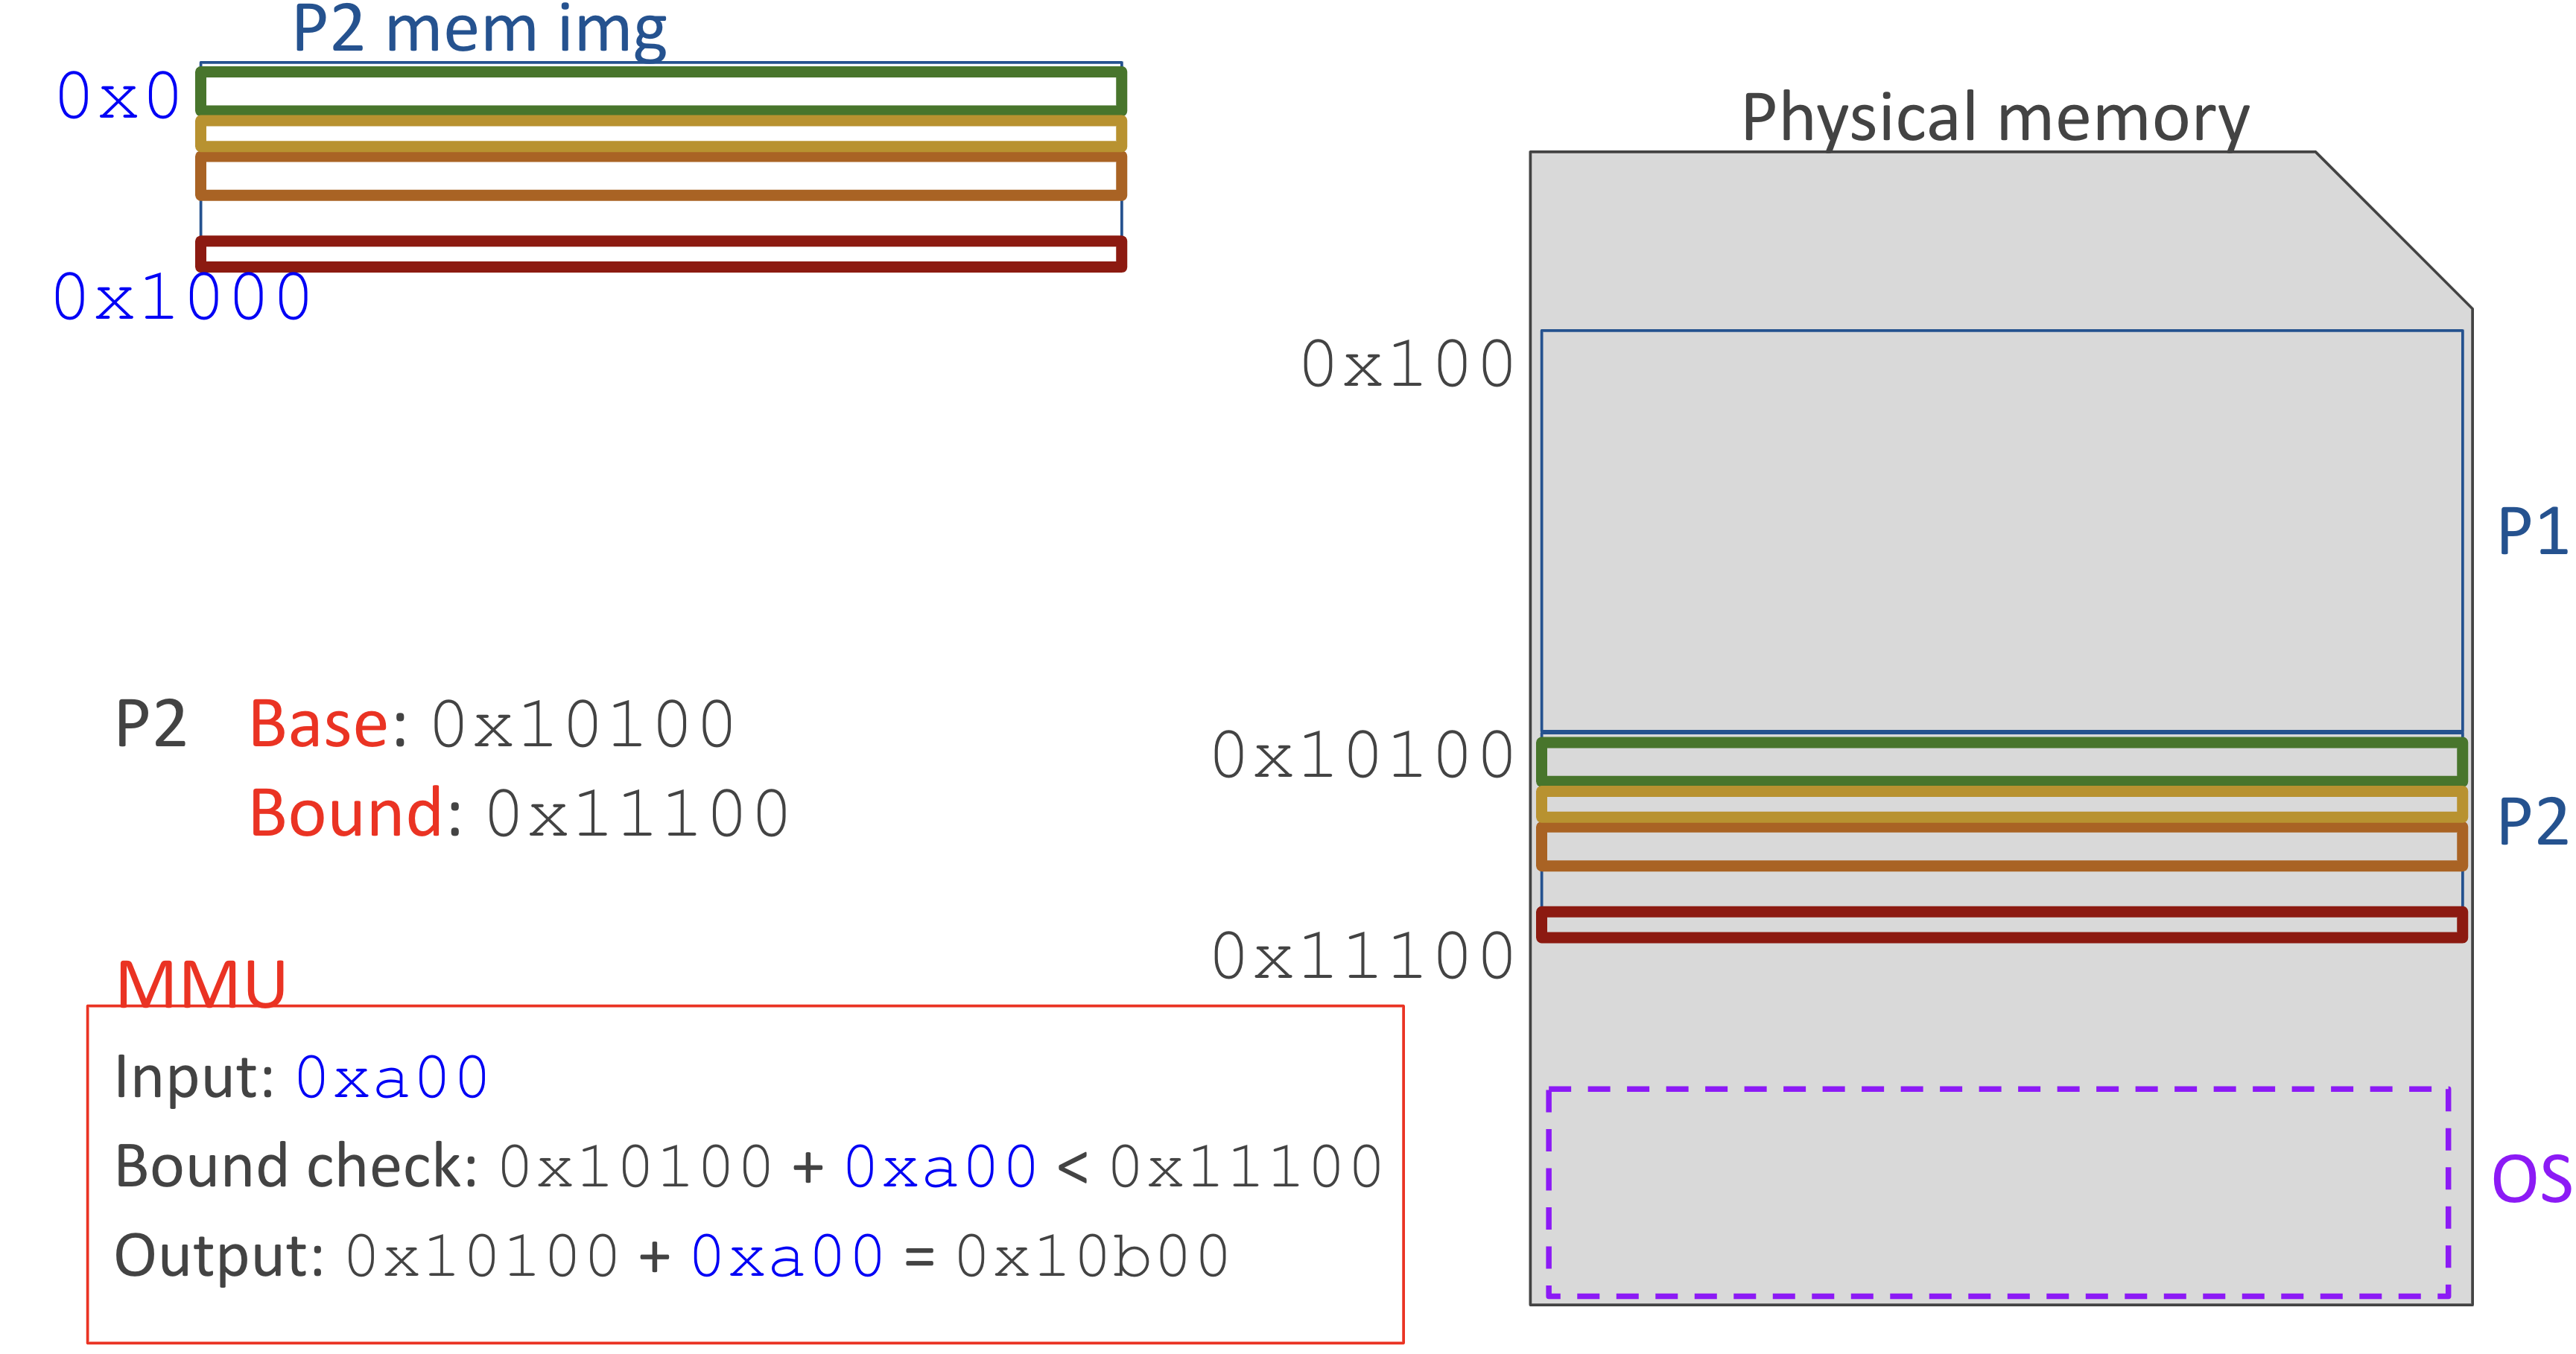
\includegraphics[width=1.1\textwidth]{chapters/L4/images/indirection-P2.png}
\end{center}
\end{minipage}
\\[70px]

\noindent In this \textbf{base--bound} scheme, each process’s memory image starts at its base address and extends just before its bound address. This approach is \textit{safe} (preventing a process from accessing memory outside its allocation) and preserves the \textit{illusion} of owning the entire memory. \\[3px]

However, because each process must reside in one contiguous memory block, \textbf{fragmentation} can occur. \\[15px]
\noindent
\begin{minipage}{0.45\textwidth}
For example, when process \(P_1\) terminates, it might leave a gap that is too small for a new process \(P_3\), even if the total available memory is sufficient.
\end{minipage}%
\hfill
\vline
\hfill
\begin{minipage}{0.45\textwidth}
\begin{center}
  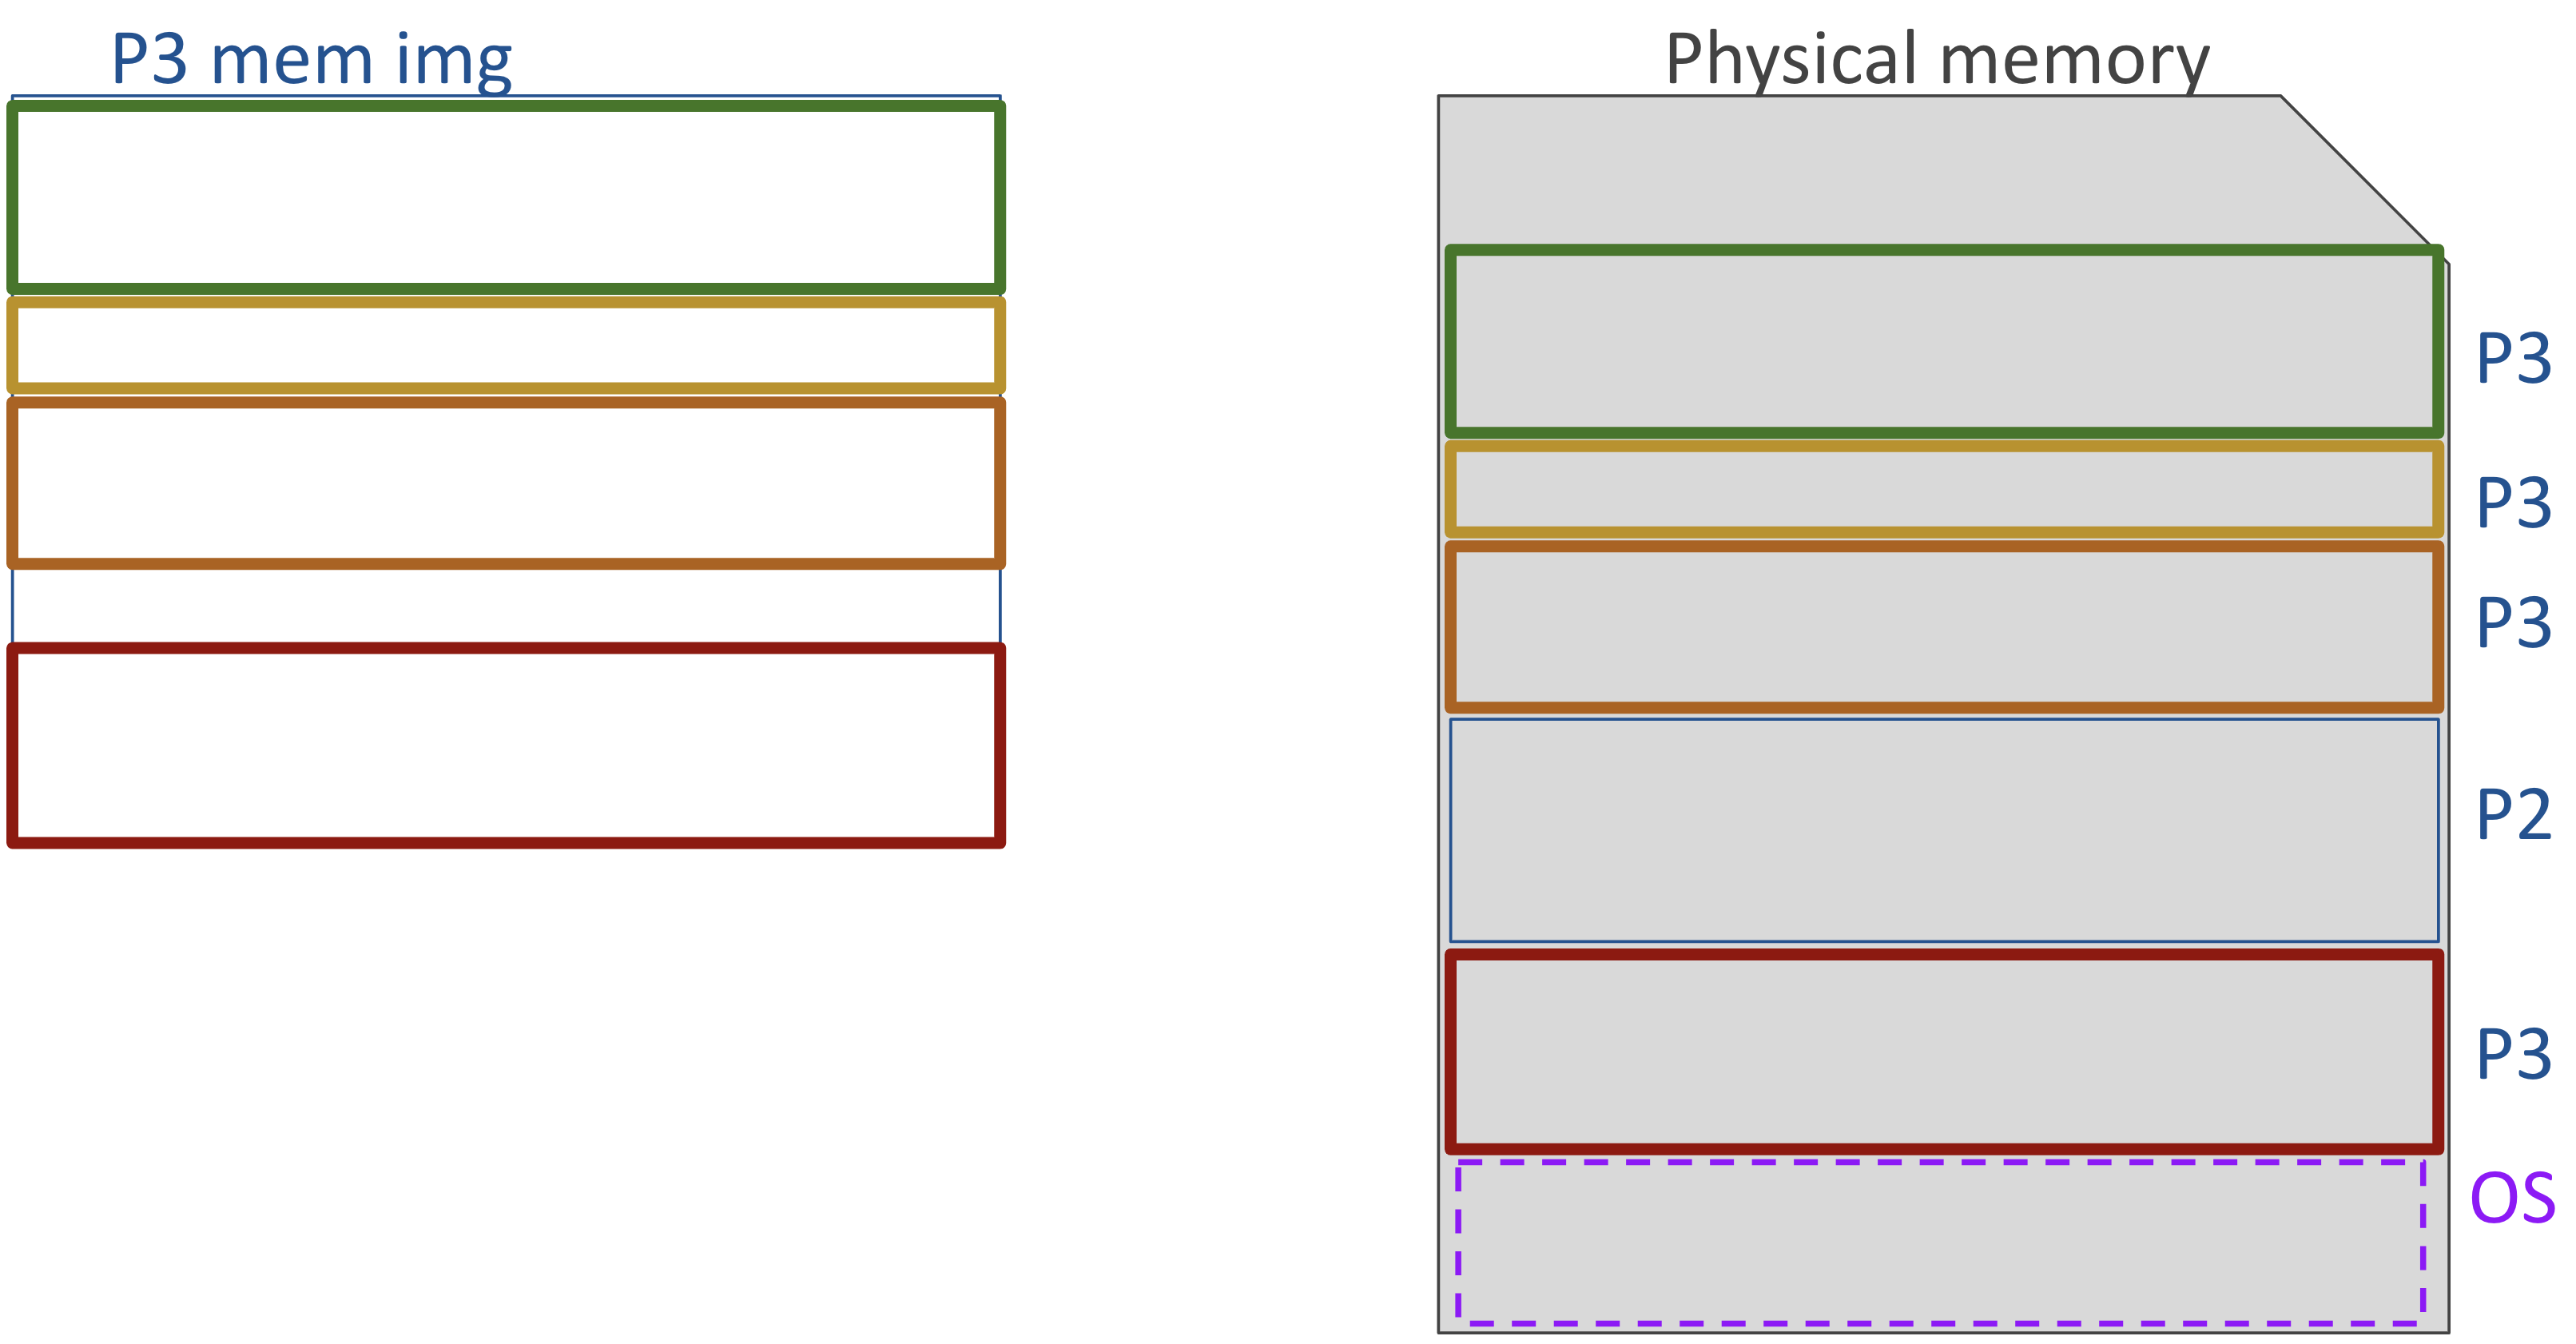
\includegraphics[width=1.25\textwidth]{chapters/L4/images/segmentation.png}
\end{center}
\end{minipage}
\\[20px]
\newpage
\noindent To address the inefficiency of requiring each process to occupy a single contiguous block of memory, an effective strategy is to \emph{divide the process’s address space into smaller chunks}, allowing noncontiguous allocation. Two primary techniques for accomplishing this are:
\vspace{10px}
\begin{itemize}
  \item[-] \textbf{Paging:} The address space is split into \emph{fixed-size pages}, which map onto equally sized \emph{physical frames}. This approach can reduce external fragmentation but can introduce \emph{internal fragmentation} if a process does not fully use the last frame of its allocation. Paging is straightforward to manage and scales well for large address spaces.
  \item[-] \textbf{Segmentation:} The address space is divided into \emph{variable-sized segments} (e.g., code, data, stack). This fits naturally with the logical structure of programs and can minimize \emph{internal} waste; however, it can result in \emph{external} fragmentation when segments cannot fit into available gaps in physical memory.
\end{itemize}

\begin{center}
  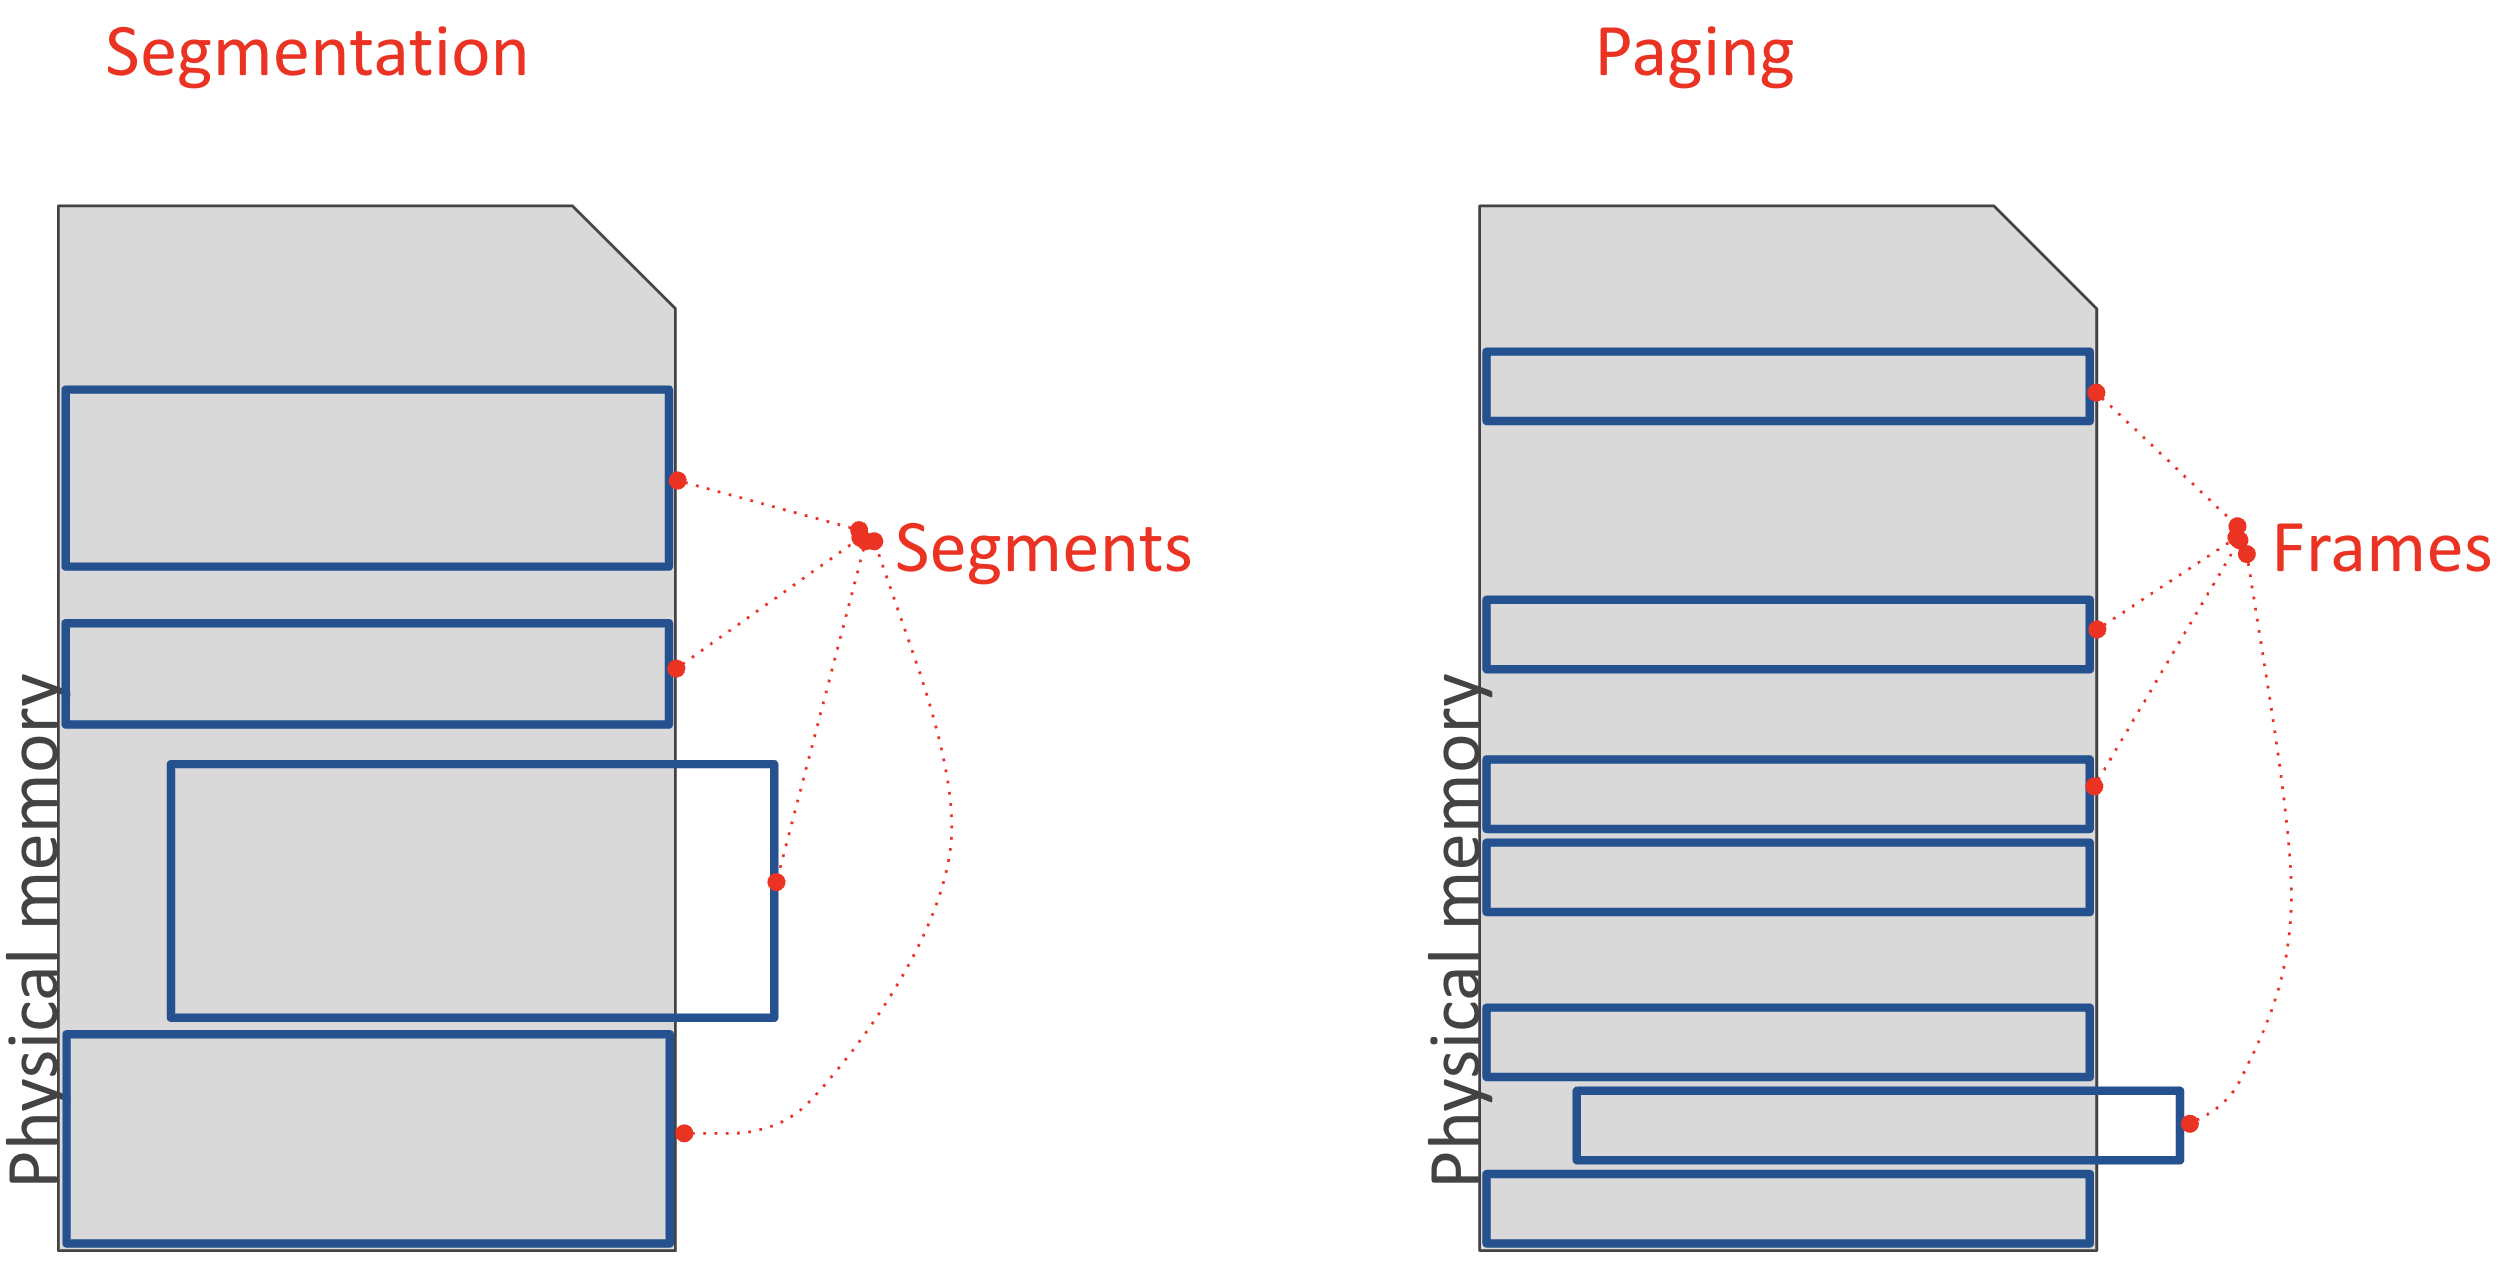
\includegraphics[width=0.65\textwidth]{chapters/L4/images/page-segment.png}
\end{center}

\noindent In \textbf{paging}, the MMU maintains a \emph{page table} to translate from virtual pages to fixed-size physical frames:

\begin{center}
  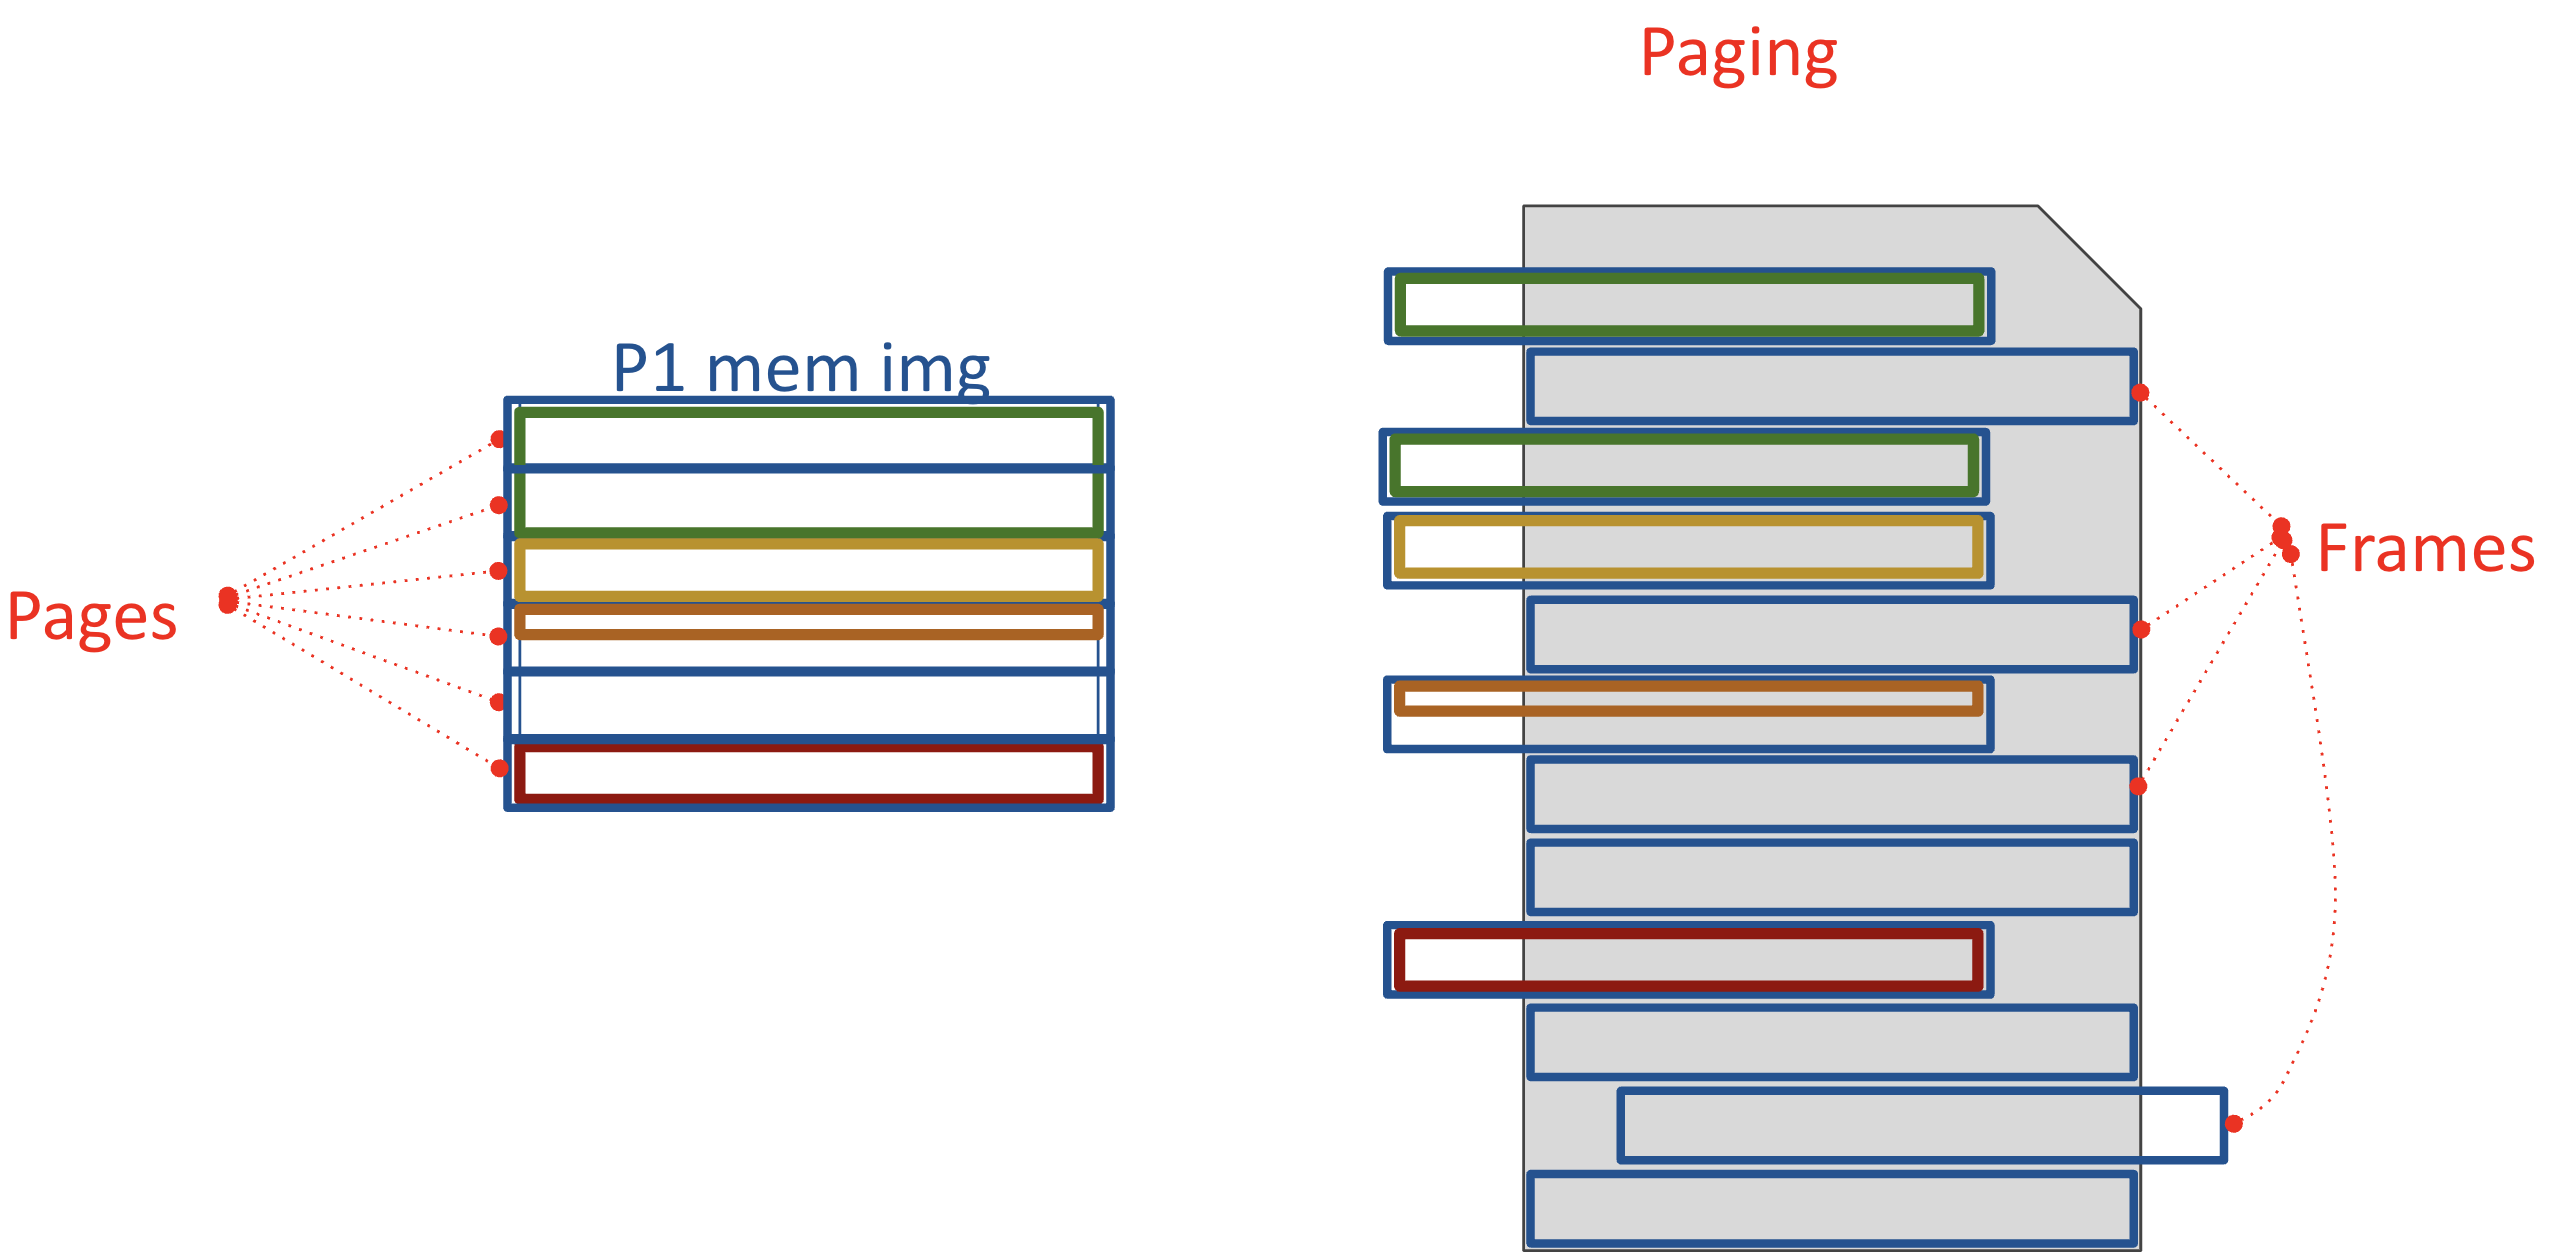
\includegraphics[width=0.65\textwidth]{chapters/L4/images/paging.png}
\end{center}

\noindent In either scheme, the MMU---\emph{configured} by the kernel with base, bound, or other address-translation structures---ensures each process can access only the memory it has been allocated. This \emph{hardware-based} translation mechanism preserves system safety and helps improve physical memory utilization by allowing noncontiguous allocation.
\newpage
\section{Optional - Operating System Mapping in Process Memory}
In modern operating systems, the OS is mapped into every process's virtual address space. This design allows a process to make system calls efficiently, as the CPU switches to pre-mapped high-address instructions during such transitions. This integration supports secure and fast interactions between user applications and system-level functions.

\begin{center}
  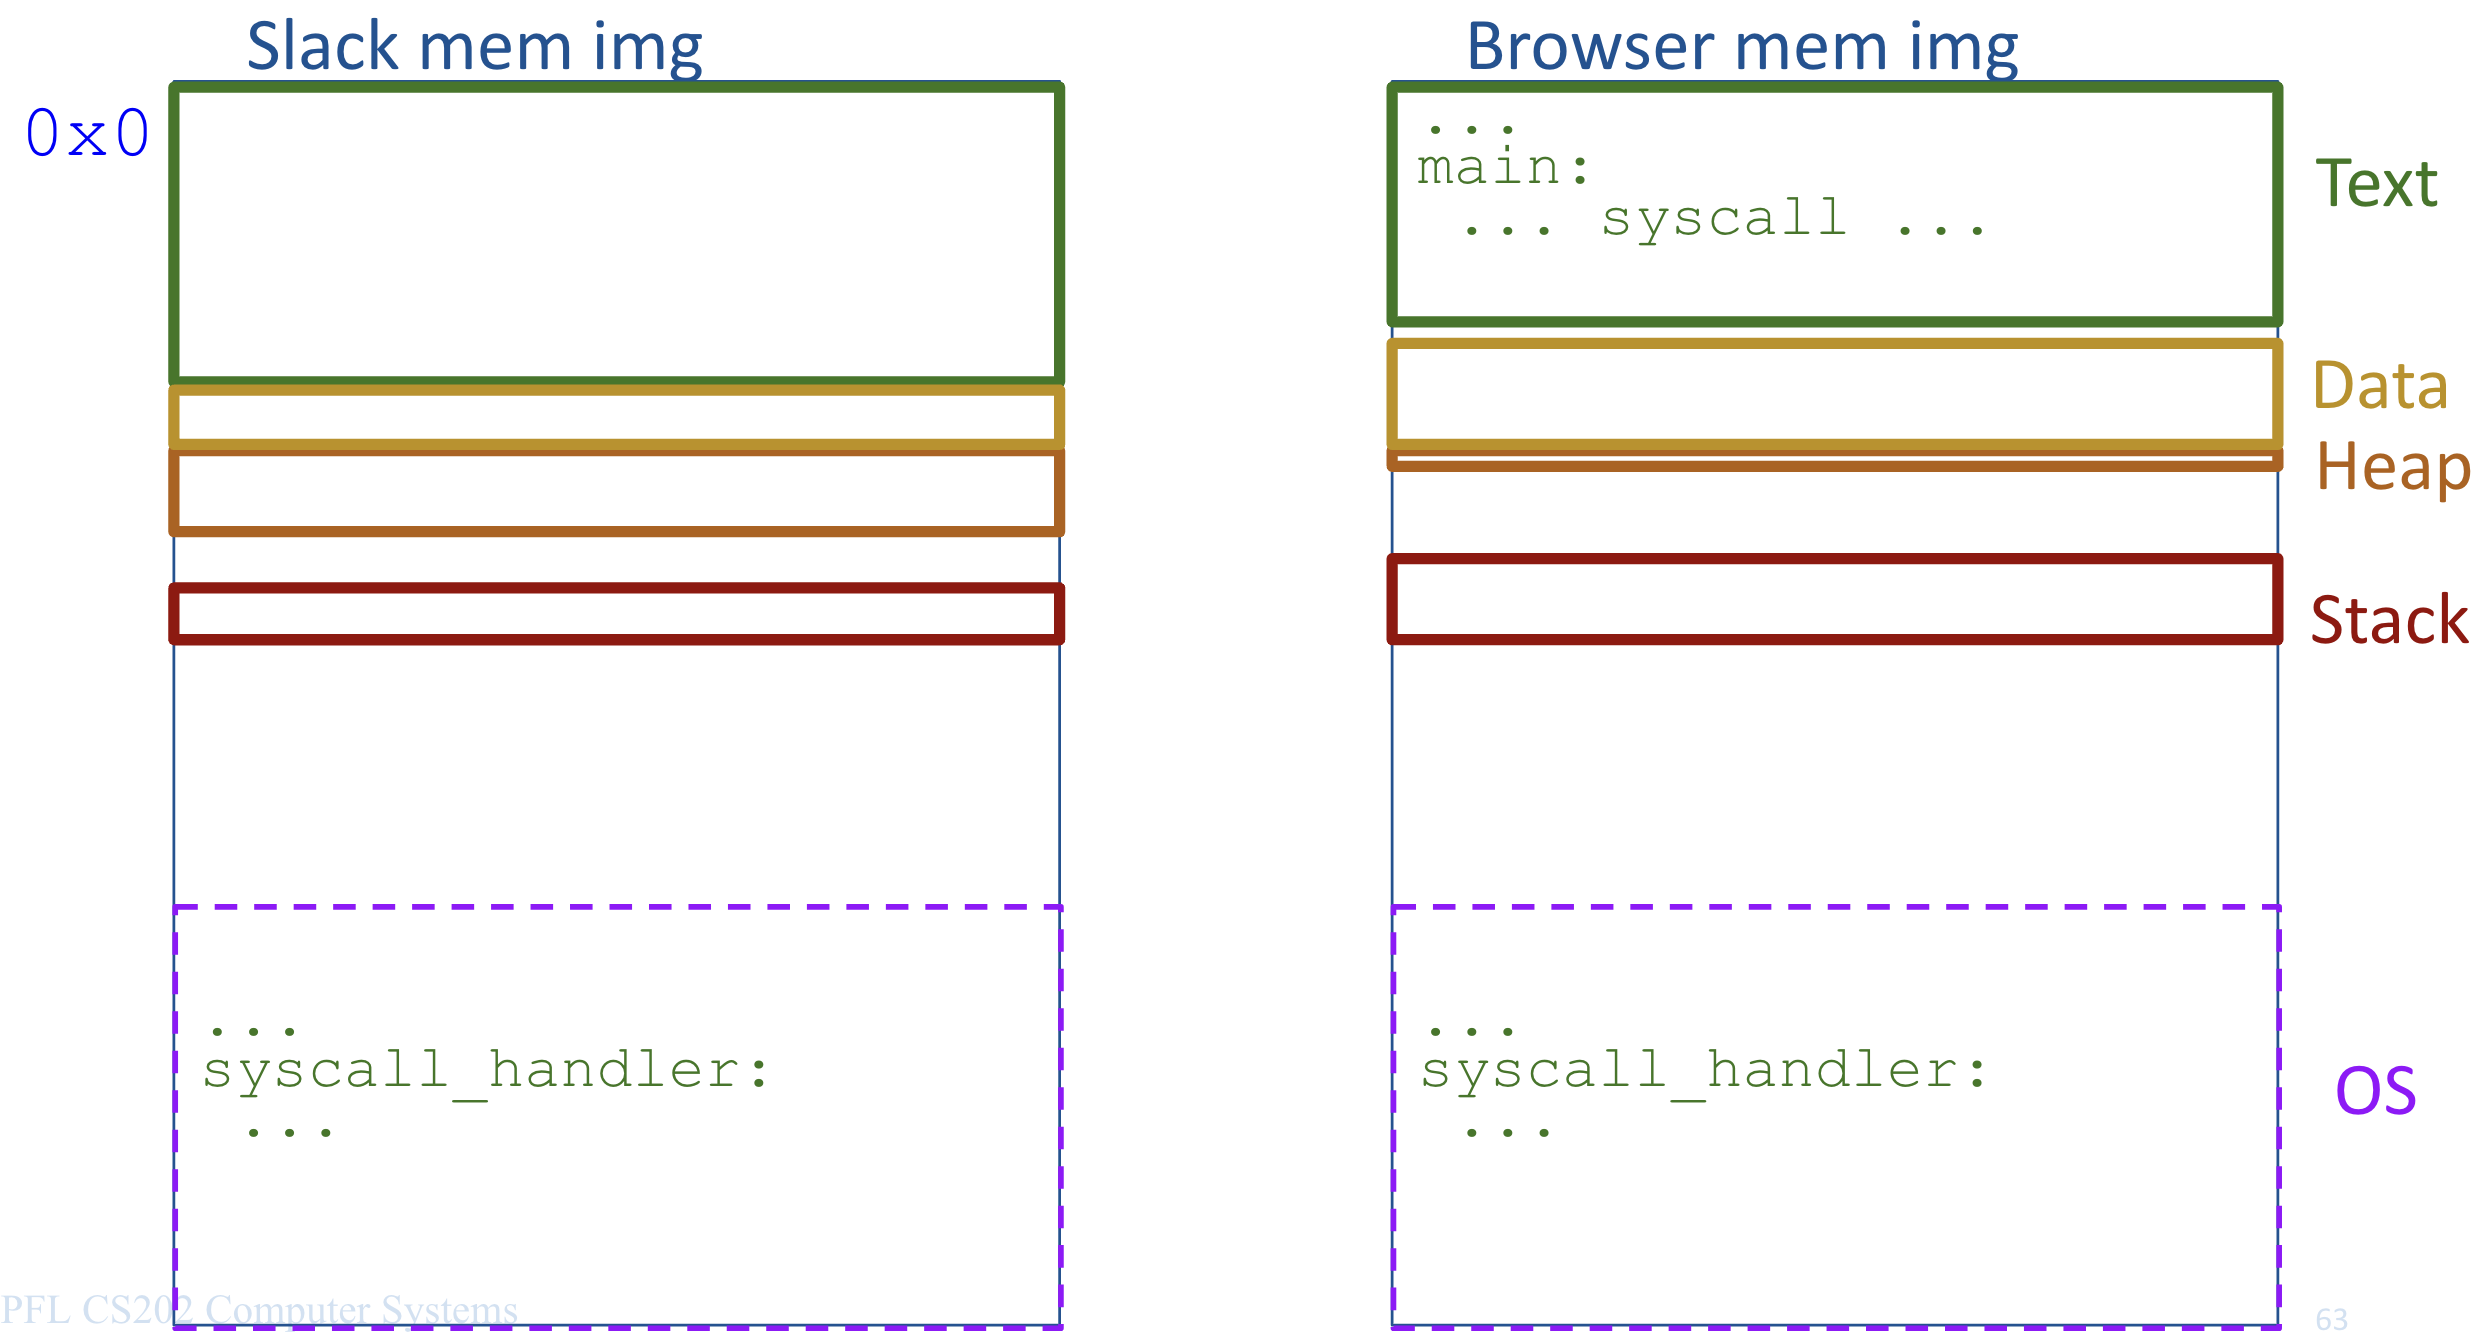
\includegraphics[width=0.55\textwidth]{chapters/L4/images/os-everywhere.png}
\end{center}

\section{CPU Caching and Memory Hierarchy}
Efficient computation in modern CPUs relies on a well-designed memory hierarchy that mitigates the performance gap between the processor and main memory. Central to this hierarchy is the CPU cache, which stores recently and frequently accessed data.

\subsection{Overview of CPU Cache}
The CPU cache is a small, high-speed memory located close to the processor core. It temporarily holds data and instructions that the CPU is likely to reuse, significantly reducing the latency compared to fetching data from main memory. This approach minimizes delays due to the slower speed of main memory and ensures smoother processor performance.
\begin{center}
  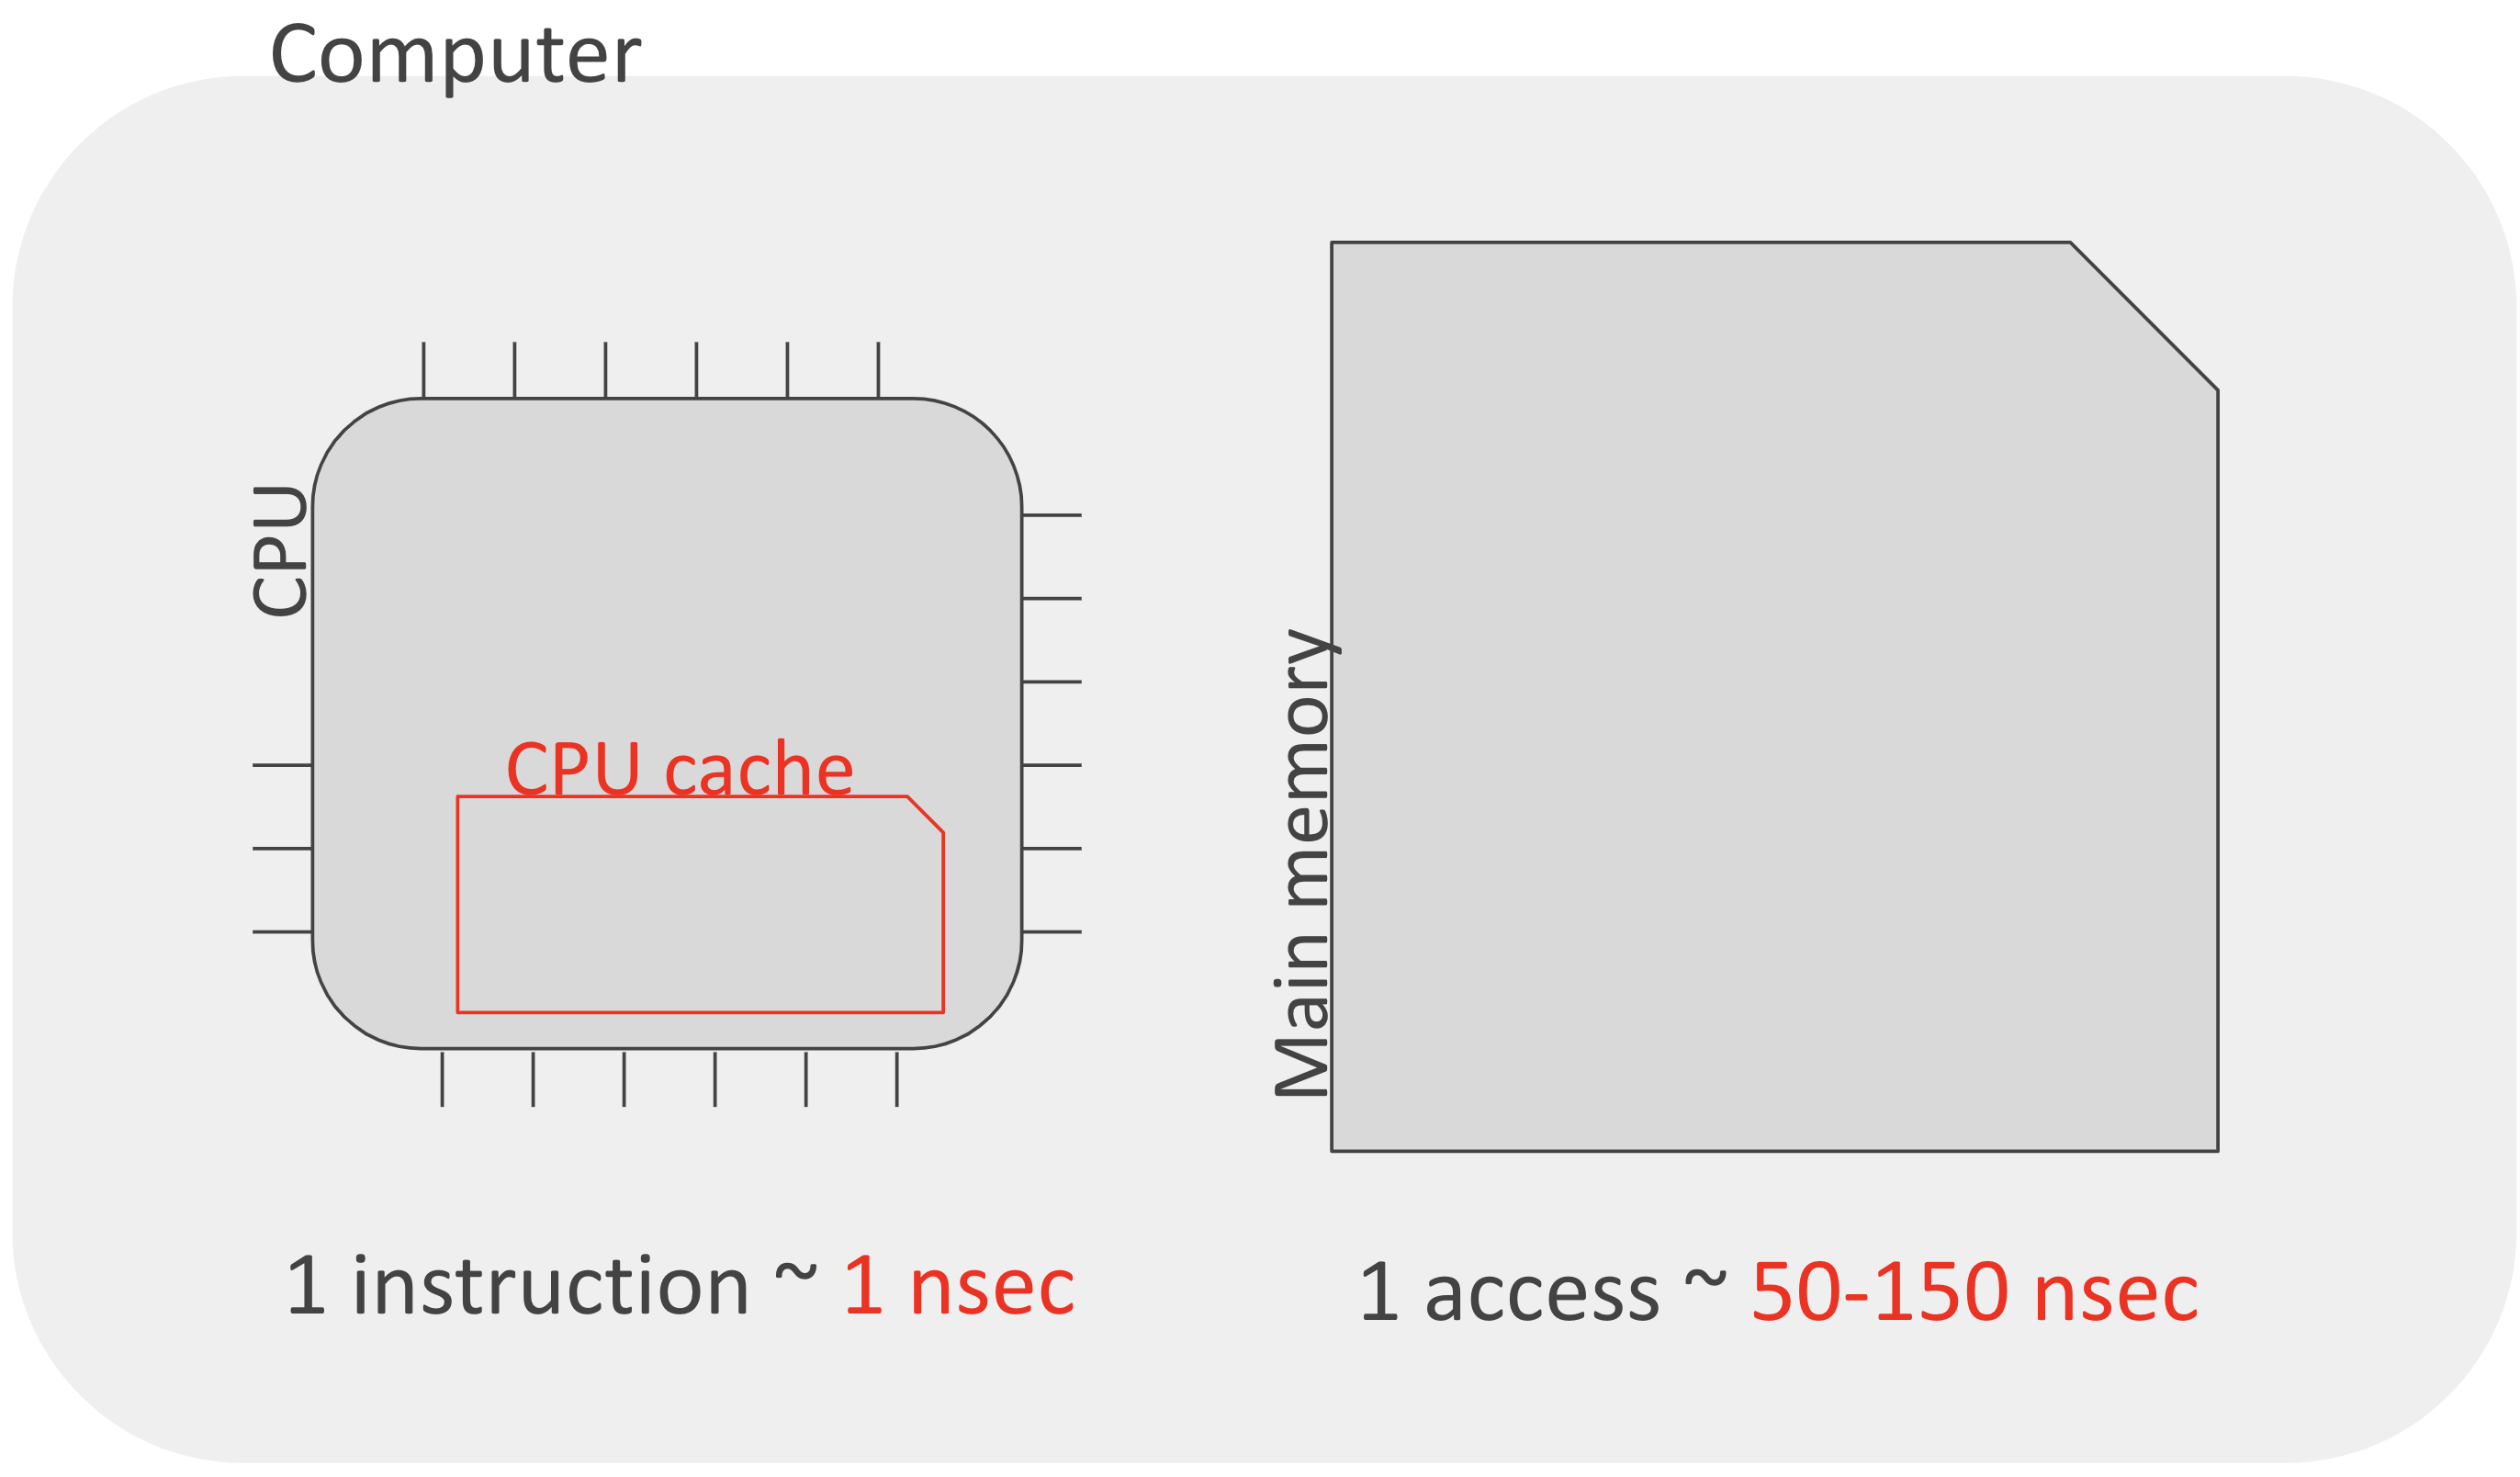
\includegraphics[width=0.55\textwidth]{chapters/L4/images/cpu-cache.png}
\end{center}

\subsection{Multi-Level Cache Architecture}
Modern CPUs employ a multi-level cache system to balance speed and storage capacity:

\begin{definition}[Cache Levels]
The cache hierarchy typically consists of:
\begin{itemize}
    \item \textbf{L\(_1\) Cache:} The smallest and fastest cache, often divided into separate instruction and data caches.
    \item \textbf{L\(_2\) Cache:} Larger than L\(_1\) and slightly slower, serving as an intermediary between L\(_1\) and L\(_3\).
    \item \textbf{L\(_3\) Cache:} The largest and slowest cache, usually shared among multiple cores in multi-core processors.
\end{itemize}
\end{definition}

The arrangement from smaller and faster (L\(_1\)) to larger and slower (L\(_3\)) reflects a deliberate trade-off between speed and capacity.

\begin{center}
  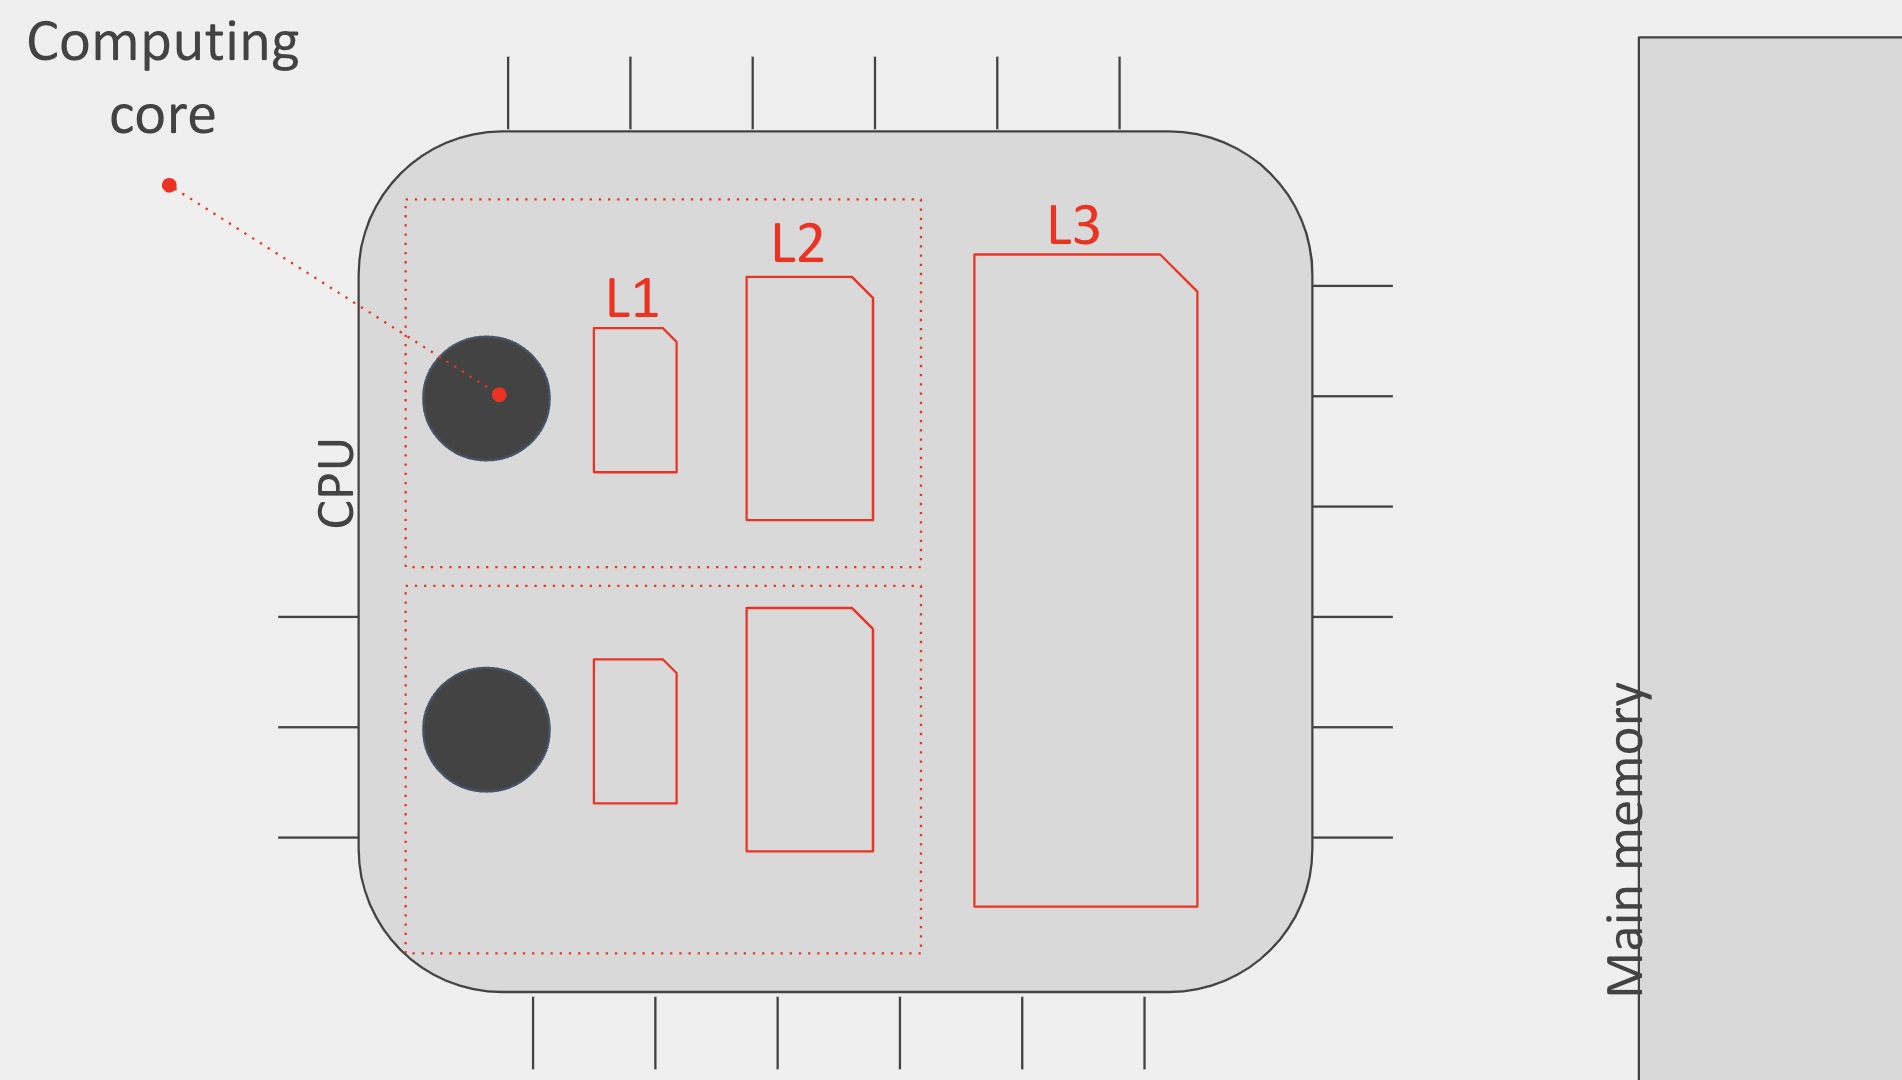
\includegraphics[width=0.55\textwidth]{chapters/L4/images/cpu-cache2.png}
\end{center}

\subsection{Cache Organization in Multi-Core Processors}
Today's processors often include multiple computing cores, each with dedicated L\(_1\) and L\(_2\) caches while sharing a common L\(_3\) cache. This design:
\begin{itemize}
    \item Provides high-speed access to data for individual cores.
    \item Balances the overall workload by reducing contention for shared resources.
\end{itemize}
Without such a hierarchical system, a single cache (e.g., L\(_1\)) might evict infrequently used yet critical instructions, thereby degrading performance.

\begin{example}
Consider a scenario in which a core with only an L\(_1\) cache continuously evicts a seldom-used, but vital instruction. The presence of additional cache levels (L\(_2\) and L\(_3\)) provides extra storage layers, ensuring that even infrequently accessed data remains available when needed.
\end{example}

\subsection{Summary of the Memory Hierarchy}
The overall memory hierarchy in a modern CPU is structured as follows:
\begin{enumerate}
    \item \textbf{L\(_1\) Cache:} Fastest, smallest, with separate instruction and data caches.
    \item \textbf{L\(_2\) Cache:} Intermediate in both size and speed.
    \item \textbf{L\(_3\) Cache:} Largest, slowest, shared among cores.
    \item \textbf{Main Memory:} Accessed only when data is not found in any cache.
\end{enumerate}
The CPU always accesses the memory hierarchy starting at the fastest level (L\(_1\)) and moving downward, ensuring that processing is carried out as efficiently as possible.
\end{document}
